% vim:ts=4:sw=4
%
% Copyright (c) 2008-2009 solvethis
% Copyright (c) 2010-2015 Casper Ti. Vector
% Public domain.
%
% 使用前请先仔细阅读 pkuthss 和 biblatex-caspervector 的文档,
% 特别是其中的 FAQ 部分和用红色强调的部分。
% 两者可在终端/命令提示符中用
%   texdoc pkuthss
%   texdoc biblatex-caspervector
% 调出。

% 采用了自定义的(包括大小写不同于原文件的)字体文件名,
% 并改动 ctex.cfg 等配置文件的用户请自行加入 nofonts 选项;
% 其它用户不用加入 nofonts 选项,加入之后反而会产生错误。
%
% 图书馆要求电子版论文的目录必须为黑色,
% 且某些教务要求打印版论文的文字部分为纯黑色而非灰度打印,
% 【因此最终打印和提交论文前,请将“colorlinks”改为“nocolorlinks”。】
\documentclass[UTF8, colorlinks, oneside]{pkuthss}

% 使用 biblatex 排版参考文献,并规定其格式。
%
% 如果无法使用 biber,可以把“backend = biber”改为“backend = bibtex”,
% 并改用 bibtex 产生参考文献,详见 pkuthss 的文档。
% 使用 biber 时,请去掉所有的 sorting 选项,否则会出错。
%
% 默认按照引用顺序排序(“sorting = none”),详见 biblatex-caspervector 的文档
% (因为是默认设置所以其实不用写,不过出于完备性的考虑仍然在这里列出)。
% 若需要按照英文文献在前,中文文献在后排序,请设置“sorting = ecnty”;
% 若需要按照中文文献在前,英文文献在后排序,请设置“sorting = centy”。
\usepackage[backend = biber, style = caspervector, utf8, sorting = none]{biblatex}
% 提供近似于学校所要求的 Times New Roman / Arial 的字体。
\usepackage[defaultsups]{newtxtext}
\usepackage{newtxmath}
% 产生 originauth.tex 里的 \square。
\usepackage{amssymb}
\usepackage{amsmath}
\usepackage{graphicx}
\usepackage{listings}
\usepackage[]{algorithm2e}
\usepackage[usenames,dvipsnames]{color}
\usepackage{xcolor}
% 按学校要求设定参考文献列表中的条目之内及之间的距离。
\setlength{\bibitemsep}{3bp}
% 对于 linespread 值的计算过程有兴趣的同学可以参考 pkuthss-extra.sty。
\renewcommand*{\bibfont}{\zihao{5}\linespread{1.27}\selectfont}

% 设定文档的基本信息。
\pkuthssinfo{
	cthesisname = {本科生毕业论文}, ethesisname = {Undergraduate Thesis},
	ctitle = {API迁移问题上的程序变换语言设计与实现}, etitle = {A Safe Transformation Language for Code Adaptation between APIs},
	cauthor = {汪成龙},
	eauthor = {Chenglong Wang},
	studentid = {1100012785},
	date = {2015.05.21},
	school = {信息科学技术学院},
	cmajor = {计算机专业}, emajor = {Computer Science},
	direction = {程序语言},
	cmentor = {熊英飞}, ementor = {Prof.\ Yingfei Xiong},
	ckeywords = {程序语言,程序变换}, ekeywords = {Programming languages, Program transformation}
}
% 载入参考文献数据库(注意不要省略“.bib”)。
\addbibresource{thesis.bib}

% 普通用户可删除此段。
\usepackage{color}
\def\pkuthssffaq{%
	\emph{\textcolor{red}{pkuthss 文档模版最常见问题:}}

	在最终打印和提交论文之前,
	请将 pkuthss 文档类选项中的 %
	\texttt{colorlinks} 改为 \texttt{nocolorlinks},
	因为图书馆要求电子版论文的目录必须为黑色,
	且某些教务要求打印版论文的文字部分为纯黑色而非灰度打印。

	\texttt{\string\cite}、\texttt{\string\parencite} %
	和 \texttt{\string\supercite} 三个命令分别产生%
	未格式化的、带方括号的和上标且带方括号的引用标记:%
	\cite{test-en},\parencite{test-zh}、\supercite{test-en, test-zh}。

	若要避免章末空白页,请在调用 pkuthss 文档类时加入 \texttt{openany} 选项。

	如果编译时不出参考文献,
	请参考 \texttt{texdoc pkuthss}“问题及其解决”一章
	“其它可能存在的问题”一节中关于 biber 的说明。
}

\newcommand{\code}[1]{\texttt{\footnotesize #1}}
\newcommand{\flyingbox}[1]{\begin{flushleft}\fbox{{#1}}\end{flushleft}}
\newcommand{\todo}[1]{{\bf \{TODO: {#1}\}}}
\newcommand{\figref}[1]{{图.\ref{#1}}}
\newtheorem{theorem}{Theorem}
\newtheorem{lemma}{Lemma}
\newtheorem{definition}{Definition}
\newtheorem{property}{Property}
\usepackage{bussproofs}
\usepackage{stackengine}
\EnableBpAbbreviations
\usepackage[all,cmtip]{xy}

\newsavebox{\fmbox}
\newenvironment{fmpage}[1]
{\begin{lrbox}{\fmbox}\begin{minipage}{#1}}
{\end{minipage}\end{lrbox}\fbox{\usebox{\fmbox}}}

\newenvironment{smpage}[1]
{\begin{lrbox}{\fmbox}\begin{minipage}{#1}}
{\end{minipage}\end{lrbox}\usebox{\fmbox}}

\newcommand{\textcd}[1]{\text{\scriptsize\BeraMonottfamily{#1}}}

\lstdefinestyle{patl}{ % Define a style for your code snippet, multiple definitions can be made if, for example, you wish to insert multiple code snippets using different programming languages into one document
%backgroundcolor=\color{highlight}, % Set the background color for the snippet - useful for highlighting
basicstyle=\footnotesize\ttfamily, % The default font size and style of the code
breakatwhitespace=false, % If true, only allows line breaks at white space
breaklines=true, % Automatic line breaking (prevents code from protruding outside the box)
captionpos=b, % Sets the caption position: b for bottom; t for top
commentstyle=\usefont{T1}{pcr}{m}{sl}\color{DarkGreen}, % Style of comments within the code - dark green courier font
deletekeywords={}, % If you want to delete any keywords from the current language separate them by commas
%escapeinside={\%}, % This allows you to escape to LaTeX using the character in the bracket
firstnumber=1, % Line numbers begin at line 1
frame=none, % Frame around the code box, value can be: none, leftline, topline, bottomline, lines, single, shadowbox
frameround=tttt, % Rounds the corners of the frame for the top left, top right, bottom left and bottom right positions
keywordstyle={[1]\color{blue!90!black}},
keywordstyle={[3]\color{red!80!orange}},
morekeywords={}, % Add any functions no included by default here separated by commas
numbers=left, % Location of line numbers, can take the values of: none, left, right
numbersep=3pt, % Distance of line numbers from the code box
numberstyle=\tiny\color{Gray}, % Style used for line numbers
rulecolor=\color{black}, % Frame border color
showstringspaces=false, % Don't put marks in string spaces
showtabs=false, % Display tabs in the code as lines
stepnumber=1, % The step distance between line numbers, i.e. how often will lines be numbered
tabsize=2, % Number of spaces per tab in the code
}
\lstset{escapeinside={@}{@}}

\lstdefinestyle{java}{ % Define a style for your code snippet, multiple definitions can be made if, for example, you wish to insert multiple code snippets using different programming languages into one document
%backgroundcolor=\color{highlight}, % Set the background color for the snippet - useful for highlighting
basicstyle=\footnotesize\ttfamily, % The default font size and style of the code
breakatwhitespace=false, % If true, only allows line breaks at white space
breaklines=true, % Automatic line breaking (prevents code from protruding outside the box)
captionpos=b, % Sets the caption position: b for bottom; t for top
commentstyle=\usefont{T1}{pcr}{m}{sl}\color{DarkGreen}, % Style of comments within the code - dark green courier font
deletekeywords={}, % If you want to delete any keywords from the current language separate them by commas
%escapeinside={\%}, % This allows you to escape to LaTeX using the character in the bracket
firstnumber=1, % Line numbers begin at line 1
frame=none, % Frame around the code box, value can be: none, leftline, topline, bottomline, lines, single, shadowbox
frameround=tttt, % Rounds the corners of the frame for the top left, top right, bottom left and bottom right positions
keywordstyle={[1]\color{blue!90!black}},
keywordstyle={[3]\color{red!80!orange}},
morekeywords={}, % Add any functions no included by default here separated by commas
numbers=left, % Location of line numbers, can take the values of: none, left, right
numbersep=3pt, % Distance of line numbers from the code box
numberstyle=\tiny\color{Gray}, % Style used for line numbers
rulecolor=\color{black}, % Frame border color
showstringspaces=false, % Don't put marks in string spaces
showtabs=false, % Display tabs in the code as lines
stepnumber=1, % The step distance between line numbers, i.e. how often will lines be numbered
tabsize=2, % Number of spaces per tab in the code
}
\lstset{escapeinside={@}{@}}

\begin{document}
	% 以下为正文之前的部分,默认不进行章节编号。
	\frontmatter
	% 此后到下一 \pagestyle 命令之前不排版页眉或页脚。
	\pagestyle{empty}

	% 自动生成标题页。
	\maketitle
	% 版权声明。
	% vim:ts=4:sw=4
%
% Copyright (c) 2008-2009 solvethis
% Copyright (c) 2010-2015 Casper Ti. Vector
% All rights reserved.
%
% Redistribution and use in source and binary forms, with or without
% modification, are permitted provided that the following conditions are
% met:
%
% * Redistributions of source code must retain the above copyright notice,
%   this list of conditions and the following disclaimer.
% * Redistributions in binary form must reproduce the above copyright
%   notice, this list of conditions and the following disclaimer in the
%   documentation and/or other materials provided with the distribution.
% * Neither the name of Peking University nor the names of its contributors
%   may be used to endorse or promote products derived from this software
%   without specific prior written permission.
%
% THIS SOFTWARE IS PROVIDED BY THE COPYRIGHT HOLDERS AND CONTRIBUTORS "AS
% IS" AND ANY EXPRESS OR IMPLIED WARRANTIES, INCLUDING, BUT NOT LIMITED TO,
% THE IMPLIED WARRANTIES OF MERCHANTABILITY AND FITNESS FOR A PARTICULAR
% PURPOSE ARE DISCLAIMED. IN NO EVENT SHALL THE COPYRIGHT HOLDER OR
% CONTRIBUTORS BE LIABLE FOR ANY DIRECT, INDIRECT, INCIDENTAL, SPECIAL,
% EXEMPLARY, OR CONSEQUENTIAL DAMAGES (INCLUDING, BUT NOT LIMITED TO,
% PROCUREMENT OF SUBSTITUTE GOODS OR SERVICES; LOSS OF USE, DATA, OR
% PROFITS; OR BUSINESS INTERRUPTION) HOWEVER CAUSED AND ON ANY THEORY OF
% LIABILITY, WHETHER IN CONTRACT, STRICT LIABILITY, OR TORT (INCLUDING
% NEGLIGENCE OR OTHERWISE) ARISING IN ANY WAY OUT OF THE USE OF THIS
% SOFTWARE, EVEN IF ADVISED OF THE POSSIBILITY OF SUCH DAMAGE.

\chapter*{版权声明}
\thispagestyle{empty}

任何收存和保管本论文各种版本的单位和个人,
未经本论文作者同意,不得将本论文转借他人,
亦不得随意复制、抄录、拍照或以任何方式传播。
否则一旦引起有碍作者著作权之问题,将可能承担法律责任。

% 若需排版二维码,请将二维码图片重命名为“barcode”,
% 转为合适的图片格式,并放在当前目录下,然后去掉下面 3 行的注释。
%\vfill\noindent
%\includegraphics[height = 5em]{barcode}



	% 此后到下一 \pagestyle 命令之前正常排版页眉和页脚。
	\cleardoublepage
	\pagestyle{plain}
	% 重置页码计数器,用大写罗马数字排版此部分页码。
	\setcounter{page}{0}
	\pagenumbering{Roman}

	% 中英文摘要。
	% vim:ts=4:sw=4
%!TEX root=../thesis.tex
% Copyright (c) 2014 Casper Ti. Vector
% Public domain.

\begin{cabstract}
	现代软件的开发离不开对于API的依赖,API的版本升级问题,以及对于API需求变化带来的API迁移问题就成为了软件维护的一个重要问题。在大规模的软件开发过程中,手动维护会极大的增加软件的维护成本,同时较高的错误率也导致了其他维护问题的产生。因此,能够快速的开发一个能够保证程序变换正确性的自动化工具就成为了软件维护者的梦想。

	然而,API之间复杂的映射,尤其是多对多的API调用映射关系,让自动转换工具的开发变得尤为困难。本文设计了一种领域特定语言(Domain Specific Language)来解决因API问题而进行程序改写的问题,通过语言机制来保证了API迁移过程中的程序变换的正确性,同时提供了用户友好的映射规则定义接口。本文定义了该程序变换语言的表里语义:表语义为用户书写转换规则过程中对于API规则的理解,而里语义则是转换规则在程序变换过程中的作用法则,并通过程序分析的手段来自动分析API转换规则在用户程序中的依赖关系,让程序的表里语义能够在实际转换过程中起到等同的作用,以此来保证变换过程在符合语言使用者理解的条件下自动推广到复杂的显示情况中。
\end{cabstract}

\begin{eabstract}
	Modern software development can not progress without the use of APIs, and this makes incompatible API update or API switching become an important but tough task for software maintainers. It is not feasible for programmers to manually update these programs between the APIs, as errors are likely to appear with manual effort, which even increases the cost of software maintenance. Thus it is desirable to have automatic program transformation tools to support the program transformation process that can maintaining the safety of the transformation process.

	To make the transformation tool programming easier, we designed a domain specific language PATL, which providing safe checks in the language semantics with user-friendly interface. In the language design, we provide an external semantics, which enables users to understand the rules they write easily, as well as an internal semantics for the actual transformation of user programs that can handle complex program transformation cases. The magic between the two semantics is the design of an analysis system which support semantic-preserving program rewriting before adaptation, which actually achieves the goals to enable users to transform complex programs with their simple rules written with the understanding of the external semantics.
\end{eabstract}


	% 自动生成目录。
	\tableofcontents

	% 以下为正文部分,默认要进行章节编号。
	\mainmatter
	% 序言。
	% vim:ts=4:sw=4
% Copyright (c) 2014 Casper Ti. Vector
% Public domain.
%!TEX root=../thesis.tex

\specialchap{序言}
% 中文测试文字。
现代的程序开发过程大量的依赖着对于API(Application Programming Interfaces,应用程序接口)的使用,因而在程序中进行API的替换也成为了程序开发过程以及软件维护过程中开发者的一项重要工作。其中,程序中的API改写主要可以分为以下两个类别。第一类是API的升级:当一个API推出的新版接口并不兼容旧版API接口时,使用旧版API的用户程序就需要进行改写来满足对于新API的使用。另一类则是API的切换,这一类情况常常出现在用户希望将原有的应用程序迁移到另一个平台上(例如从Android到IOS的程序切换),或是因为对于API性能以及维护功能上的其他需求而要求将原有的API切换到另一个API集合中去。在以上描述的这两种API更替场景中,我们需要将使用$API_1$的程序变换为使用$API_2$的程序,而$API_1$与$API_2$之间具有同构性,这样的替换也即相同功能之间的不同接口替换。然而,这样的程序变换并不容易。当用户手动进行这样的程序转换时,由于并非所有用户都是API的专家,他们并不能够全盘掌握两个API之间的映射关系,以及难以顾及到不同转换之间的交叉问题,手工的转换带来的结果就常常是错漏连篇的新程序,这带来结果就是更加高昂的软件维护成本和更多的人力资源消耗。

既然对于API升级的程序改写如此重要而又如此困难,让API发布者提供一个自动的程序转换工具就成为了帮助客户端程序员(即使用API的用户程序员)进行程序升级的一大利器:当API进行更新的时候,API发布者在发布API库的时候同时提供了一个用户升级工具来帮助客户进行程序升级,用户只需要让工具自动的将原有的程序进行改写就成为了使用新API的程序。让API提供者开发这样的转换工具具有相当的好处:一方面,作为API的专家,他具有更加丰富的API映射关系的知识,他能够处理还API之间的多方面映射关系,而另一方面,这样工具的开发是独立于用户程序的,一次开发就能够让广大用户都可以进行程序的升级,可以广泛的解决用户的需求问题。这样的工具例子有1)微软为了推广自己的.Net平台,提供了Visual Basic到Visual Basic.Net的程序转换工具,2)RIM提供了一个从Android到Blackberry的平台迁移工具,让使用Android API的程序能够自动改写为使用Blackberry的工具,从而可以让转换后的程序在Blackberry上运行而不需更多的工作。

然后,开发这样的Source-to-source自动转换工具并不容易。从转换工具的市场上来看,只有极小的一部分API拥有了这样的自动转换工具来完成程序的改写工作,其中一个重要的原因就是这些API间的程序自动转换工具常常会引入一些新的错误,或是在具体的程序环境中并不能完全按照API开发者的意图进行程序之间的改写。其中一个典型的例子就是Python 2to3.script工具,这个工具是设计来将使用python 2.x版本的程序升级为使用python 3.x版本的程序。虽然这个升级脚本能够在一定程度上完成对于python API的升级工作,但在升级过程中也引入了较多的错误,在有Pilgrim与Willison的案例研究\cite{python}中,2to3.script会导致包括类型错误在内的很多程序错误。从另一方面来看,程序变换开发的困难源自于专业开发环境的支持。由于并非所有的API开发者都能够熟悉程序语言的修改操作,让他们从底层开始实现这样的转换工具就显得困难重重。

事实上,为了解决程序变换的难题,程序语言社区设计出了很多的程序变换语言\cite{twinning}\cite{stratego}\cite{txl}。这些语言通过高层次的抽象来帮助使用者避开了底层开发中容易产生的错误,例如转换语言中能够保证程序变换前后不会产生语法错误,同时能够帮助开发者更好的描述自己需要表达的转换对象。然而对于API迁移这样一个特定场景的问题,这些变换语言的设计就显出了明显的不足,主要体现在以下几个方面:
\begin{itemize}
\item API变换过程中的类型安全并没有得到保证:这些通用的程序变换语言由于广泛的解决了多类的程序变换问题,类型安全就显得难以控制,而在较为单一的API升级问题中,变换对象保持在了statement以及expression层次上,类型的正确性就变得可控同时具有高层次的操作性。
\item API之间的映射没有得到高层次的抽象,因而这些转换仍然需要较多对于用户context的明确指定。由于API转换工具开发者需要能够在未知用户程序环境的情况下完成映射规则的指定,复杂的context就难以得到实现。
\item API升级之中多对多的API映射没有得到良好的支持:API之间的多对多问题涉及到了程序之间的环境分析问题以及转换语句之间的依赖关系问题,而大多数变换语言都是从语形上进行的转换,这样的转换就忽略了转换对象在运行时候的以来关系以及对应关系,从而导致了变换过程的实际语义遭到了违反。
\end{itemize}

我们接下来通过几个实际的例子来描述API之间程序改写中的常见问题。
\paragraph{类型安全问题} 类型安全问题主要体现在程序迁移前是类型正确的而改写之后出现了类型错误,举例如下。(该案例来自\cite{swing2swt})

在Java图形界面编程API Swing到SWT的升级过程中,Swing在创建一个窗口时需要首先创建一个Container来存放窗口中的内容,SWT也同理需要创建一个对应的Composite类来进行存放。(类图见\figref{swing2swtfig})因此在升级过程就就有了这样的两条对应关系(此处的规则只是简单的描述了API之间的映射关系,其中的$\pi_1$可以读作“将\code{Container}类的构造函数映射到\code{Composite}的构造函数,其中\code{Composite}的构造函数参数为\code{new Shell()}以及0”,第二条规则则是将\code{JList}类映射到\code{List}类,并将其构造函数进行对应的替换。):
\[
\begin{array}{ll}
	\pi_1=\code{new Container() ->> new Composite(new Shell(),0)}\\
	\pi_2=\code{new JList() ->> new List()}
\end{array}
\]
\begin{figure}[ht]
\centering
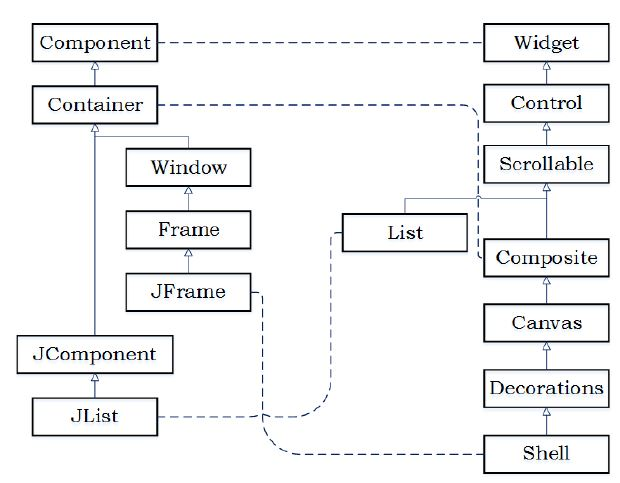
\includegraphics[width=200pt]{fig//swing2swt_class.JPG}
\caption{Swing(图左)到SWT(图右)之间的类图对应关系,其中虚线箭头表示两个API之间的类映射,实线箭头表示同一API中类的继承关系(往下为父类)}
\label{swing2swtfig}
\end{figure}
在这样的转换规则下,用于转换如下用户程序时就会出现类型的错误。
\[
\code{JList list = new Container();} \longrightarrow \code{List list = new Composite(new Shell(), 0);}
\]
其原因在于在\figref{swing2swtfig}中,Swing类型中的JList是Container的父类,因而左部满足子类关系而右部的List不再是Composite的子类,因而转换之前的类型是正确的,而转换之后就会导致类型错误的出现。

\paragraph{API之间多对多的映射问题}
比起前面所提到的类型问题,程序变换中更复杂的多对多问题更为引人注目。API之间多对多映射带来的主要问题则是用户程序上下文之间的不一致性,这样的问题并不像类型错误那样能够通过静态检查就能够得到并修复,而复杂的runtime错误让这类问题更容易隐藏。

在这里我们先简单使用程序匹配语言SmPL\cite{spatch}的语法来展示变换的规则。
\begin{center}
\begin{smpage}{0.25\columnwidth}
\begin{lstlisting}[style=patl]
(a:A->B) {
	- a.x();
	- a.y();
	+ a.z();
}
\end{lstlisting}
\end{smpage}
\end{center}
这一条规则就代表了一组API到另一组API之间的映射,元变量定义部分的\code{a:A->A}就代表了元变量在原来的API集合中类型为A,在新的API集合中类型为B,而这条规则表示了“每当遇到一个类型为A的变量a连续调用了a.x()与a.y()两个方法,我们就删除这两条语句,并用a.z()这样的一条语句来进行替换。”

假设我们现在的转换空间具有如下两条规则:
\begin{center}
\begin{smpage}{0.25\columnwidth}
\begin{lstlisting}[style=patl,frame=none]
(a:A->A) {
  - a.y();
  - a.x(); 
  + a.n(); 
}
\end{lstlisting}
~~~~{\small Rule-1}
\end{smpage}
\qquad\quad
\begin{smpage}{0.35\columnwidth}
\begin{lstlisting}[style=patl,frame=none]
(a:A->A,b:int->int) {
  - b = a.z();
  - a.x();
  + b = a.m(); 
}
\end{lstlisting}
~~~~{\small Rule-2}
\end{smpage}
\end{center}
让我们来考虑如下几种实际的转换类别来分析这两个例子的具体问题。
\begin{enumerate}
\item 情形1:在同一个context可以正确转换的例子。
\begin{center}
\begin{smpage}{0.3\columnwidth}
\begin{lstlisting}[style=patl,frame=none, numbers=none]
a.y();
a.x();
\end{lstlisting}
\end{smpage}
\begin{smpage}{0.6\columnwidth}
\begin{lstlisting}[style=patl,frame=none, numbers=none]
if (true) {
  a.y();
  a.x();
} else {
  b = a.z();
  a.x(); }
\end{lstlisting}
\end{smpage}
\end{center}
在这两个例子中,用户规则可以直接的在一个基本块中匹配到需要进行转换的语序序列,在类型和语形都能够正确匹配的情况下就能够进行正确的转换。因此可以比较容易的完成操作。
\item 情形2:被匹配的代码并不直接出现在连续块中,而需要进行调整来进行转换。
\begin{center}
\begin{smpage}{0.2\columnwidth}
\begin{lstlisting}[style=patl,frame=none, numbers=none]
b=a;
a.y();
b.x();
\end{lstlisting}
\end{smpage}
~
\begin{smpage}{0.2\columnwidth}
\begin{lstlisting}[style=patl,frame=none, numbers=none]
a.y();
i++;
a.x();
\end{lstlisting}
\end{smpage}
~
\begin{smpage}{0.48\columnwidth}
\begin{lstlisting}[style=patl,frame=none, numbers=none]
if (i<0) 
  a.y();
else 
  b = a.z();
a.x();
\end{lstlisting}
\end{smpage}
\end{center}
在上述的三个例子中,虽然并没有直接出现连续的转换指令,但是这些代码块却可以进行调整来使得代码变得可以转换。例如第一段代码中,由于\code{b}与\code{a}为alias关系,可以将\code{b.x();}重写为\code{a.x();},从而让转换可以正常进行。第二段代码中\code{i++;}与\code{a.x();}并没有依赖关系,从而可以交换位置让\code{a.y();a.x();}连续出现,因而也可以进行转换。第三段代码则可以通过将\code{a.x();}移动到两个分支语句中,从而让两个分支分别进行转换。
\item 情形3:类似于第二种情形,但是却因为以来关系的出现而无法转换。
\begin{center}
\begin{smpage}{0.44\columnwidth}
\begin{lstlisting}[style=java,frame=none, numbers=none]
b=a.z();
if (b<0) 
	a.x();
else
	a = new A();
\end{lstlisting}
\end{smpage}
\end{center}
在上面的这一段代码中,由于分支语句的条件\code{b<0}依赖于\code{b=a.z();},\code{b=a.z();}就不能像上述2-3的语句一样进行移动,从而产生了一个转换异常需要报告给用户。
\end{enumerate}

由于上述的种种困难,开发一个能够正确处理API之间程序改写的工具就显得尤为困难,因此在实际应用中,一个良好的程序转换工具应该能够保证独立于客户端程序的正确性:假设对于用户程序$p$,有一条在$p$上的性质$\phi$,那就需要对于一个转换程序$\Pi$,使得对于所有的$p$,都能够做到$\phi(p)$成立可以得出$\phi(\Pi(p))$也成立。这个关系可以形式化的表述为:
$$\forall p.\phi(p)\Longrightarrow\phi(\Pi(p))$$
在我们的目标中,我们就把性质$\phi$定义为类型正确性以及依赖关系的正确保持。
此外,让程序能够完全自动的转换任意的客户端程序而不会产生错误显然并不是一个可行的手段。实际进行程序变换的过程中,应当能够有规则检查系统来对转换程序进行检查,可以将规则的错误以及规则在非规范程序上可能产生的不正常表现报告给用户,从而让用户能够理解转换工具将在程序中进行的操作,并保证能够在所有错误正确处理的情况下就能够保证性质$\pi$的保持。这个关系可以由以下关系表示:

\begin{property}[Transformation Safety]
Given $p$,$\Pi$,if $\mathsf{check}(p,\Pi)==\code{true}$ and $\phi(p)$ holds, then $\phi(\Pi(p))$ holds, or else $\mathsf{check}(p,\Pi)$ will report warnings for the transformation.
\end{property}

除了对于转换目标正确性的支持,语言应当能够具有以下的特点以能够实际作为API之间程序变换问题的一个解决方案:
\begin{enumerate}
\item 能够高层次的描述API间的程序变换问题,表达能力要足够强,让用户能够表达绝大部分的API转换问题同时尽量减少对于非必要功能的依赖。
\item 转换规则的书写应当是独立于用户程序,需要能够保证作用在不同用户程序下都保持相同的转换特征。
\item 语言应当能够在用户程序中的API使用违反API使用规则时向用户提供错误信息,在转换前就能让用户知道需要进行修改的部分。
\end{enumerate}

本文主要就从语言机制的角度探讨了对于API之间程序改写问题的解决方案。本文设计了程序语言Patl,一种用具解决API升级问题中的多对多问题程序变换语言。本文的主要启示就在于将匹配放在了控制流图之中进行,并且在实际的程序改写之前进行一系列的语义等价转换,最后才在等价变换的程序变换基础上进行实际的API改写操作,同时在改写之中保持程序变化之间类型性质的转换正确性。

在接下来的章节中,我们首先会具体说明具体的研究问题难点,形式化的概述我们的解决方案(第一章),通过几个具体案例说明我们的解决方案(第二章),形式化的描述语言的语形语义(第三、四、五章),最后分析语言的应用以及在几个数据集下的分析结果(第六章)。


	% 各章节。
	% vim:ts=4:sw=4
% Copyright (c) 2014 Casper Ti. Vector
% Public domain.
%!TEX root=..//thesis.tex

\chapter{方法概述}
% 中文测试文字。
在上一章中,我们提出了变换语言的设计目标。我们将在本章通过几个案例来阐释Patl语言的设计。

\section{Patl的转换框架}

\subsection{表语义与里语义}

为了缩短抽象的转换规则与具体的语言作用效果的鸿沟,我们为Patl赋予了表语义与里语义。其中表语义(也即抽象语义),是为用户提供理解的转换语义,用户在书写规则时可以根据表语义来理解其转换规则在程序中的作用方式。而在表语义之外,Patl还具有里语义(即算法语义),其作用是等效的将表语义所表示的变换最大化的推广到程序的控制流图中,同时将可能违背表语义转换法则的程序部分报给给用户进行手动处理。这样设计的重要原则就是让表语义与里语义能够具有等效性,否则转换程序作用在客户端程序上的时候就会导致违背用户规则意图的效果。当表里语义做到等效作用时,用户就可以在只需最小限度的理解程序的表象效果就能够完成复杂程序上下文中作用的工作。

接下来我们将形式化的描述这个转换框架。
\begin{definition}[表语义转换]
给定一个转换程序$\Pi$,以及两个程序$p_1$,$p_2$,如果$p_2$满足:对于$p_1$中所有的被规则$\Pi$匹配的连续程序块,$p_2$中都由规则$\Pi$的映射结果替换,则我们称$p_1$与$p_2$具有表语义转换关系,我们使用符号$p_2={\Pi}\circ(p_1)$来表示。
\end{definition}

简单来说,表语义就是在引言部分所使用的“块替换”的转换方法:给定一条转换规则$\Pi=()\{-p_1;-p_2;...;-p_n;+q_1;...;+q_n\}$来转换一个程序语句序列$s_1;...;s_n$,表语义所进行的转换即是找到$s_1;...;s_n$中的一段顺序语句$s_{l_1};..;s_{l_u}$,使得这段语句匹配$p_1;...;p_n;$,然后将语句序列替换为$q_1;...;q_n$,从而使得程序中的对应片段得以转换。

\begin{definition}[里语义转换]
里语义转换定义为根据算法语义(见后文)进行的上下文有关的程序匹配替换,我们用符号$p_2=\Pi\bullet(p_1)$来表示$p_2$是$p_1$在$\Pi$的里语义下的转换结果。(作为简化,我们也常常用$\Pi(p)$来表示里语义转换)
\end{definition}

给定程序上的一个语义等价关系“$\doteq$”(即$p_1\doteq p_2$意味着$p_1$与$p_2$语义等价),我们使用下图来描述这两个转换的关系。

\begin{equation}\label{eqn:diagram}
  \xymatrix{
    q \ar[r]^{\Pi\circ}  & q' \ar@{<->}[d]^{
    \doteq} \\
     p \ar[r]_{\Pi\bullet} \ar@{<->}[u]_\doteq       & \Pi(p) }
\end{equation}

这个交换图表述了里语义与表语义之间的关系:里语义在一个程序$p$上的作用结果等价于表语义在$q$上的作用结果,而其中$q$与$p$是语义等价的两个程序。这个图的交换性就表述了Patl在里语义与表语义的设计目标:里语义与表语义的作用在等价关系$\doteq$的意义下等效(下文将在语言设计的基础上证明该图的交换性以及等价关系$\doteq$的等价性)。

此外这个等效关系也可以通过抽象解释的方式来进行阐释:首先我们将$p$到$\Pi(p)$的流程转化为$p\leftrightarrow q \rightarrow_{\Pi\circ}q'\leftrightarrow \Pi(p)$。那么,对于抽象语义函数$S$,我们持有以下关系:

\begin{displaymath}
  \xymatrix{
    p \ar@{<->}[r]^\doteq \ar[d]^S & q \ar[r]^{\Pi\circ}  \ar[d]^S & q' \ar@{<->}[r]^{
      \doteq} \ar[d]^S & \Pi(p) \ar[d]^S\\
    S(p) \ar@{<->}[r]^= & S(q) \ar@{<->}[r]^= & S(q') \ar@{<->}[r]^= & S(\Pi(p))}
\end{displaymath}

这个关系的含义也即是上图中的交换图代表的含义,意味着每一步转换都保持了语义的等效性,(其中的API迁移过程也是在保持语义下的API)从而也表示了变换框架里语义与表语义所应当具有的对应关系。

\section{Patl的转换流程}
在表述了这两种语义的基本框架后,我们就开始着重介绍里语义的转换案例,通过这样的转换案例的介绍,我们将知道转换程序具体作用在客户端程序上的表现。

在这一个章节中,我们采用如下从SWT到GWT的一个转换案例来解释语言的作用法则。这一个样例展示的是从SWT到GWT的一个表格绘制功能的转换。

两个API在此处需要完成的工作都是创建一个表格,给表格添加一些列,然后在表格的第一列添加一个单元格。

\begin{figure}[ht]
\begin{center}
\begin{smpage}{0.5\columnwidth}
  {\small (a) Source client code:}
\begin{lstlisting}[style=java]
column.setWidth(100);
TableCell cell1 = new TableCell();
column.add(cell1);
TableCell cell2 = new TableCell();
column.add(cell2);
\end{lstlisting}

  {\small (b) Target client code:}
\begin{lstlisting}[style=java]
GridCell cell1 = new GridCell(100, column);
GridCell cell2 = new GridCell(100, column);
\end{lstlisting}
\end{smpage}
\end{center}
\caption{Client code}
\label{fig:client}
\end{figure}

上图中的a)部分表示的是SWT中的规则,SWT会首先创建一个列,为列设置好宽度属性之后创建一个单元格,再将单元格加入到列中。上图的b)部分则表示了GWT的修改方式:不需要将单元格加入到列中,而是把列\code{column}以及宽度\code{100}直接作为参数传入。

给定了这样的对应关系,我们可以定义如下的两条转换规则:

\begin{figure}[ht]
\begin{center}
\begin{smpage}{0.5\columnwidth}
\begin{lstlisting}[style=patl]
/*tRow*/ ( col: TableColumn -> GridField,
       cell: TableCell -> GridCell,
       w : int -> int) {
  m col.setWidth(w);
  - cell = new TableCell();
  - col.add(cell);
  + cell = new GridCell(w, col);
}

/*tSetWidth*/ (col: TableColumn -> GridField,
           w: int -> int) {
  - col.setWidth(w);
}
\end{lstlisting}
\end{smpage}
\end{center}
\caption{Transformation program}
\label{fig:transform}
\end{figure}

这两条转换规则就表述了上述的SWT到GWT程序之间的对应关系。

\subsubsection{表语义转换规则}

根据我们前文的表语义做法,我们就会进行语形以及类型上的匹配来确立需要转换的程序片段,从而进行直接的替换。例如对于\figref{fig:client}中的例子,我们就会通过语形以及类型的匹配让这些规则与用户语句产生绑定,然后根据语句的绑定关系进行代码生成。

具体在\figref{fig:client}中,其中\code{tSetWidth}这一条规则就会使得其中的语句序列与设置宽度的语句产生绑定,而\code{tRow}这条语句能够让添加单元格的语句进行匹配。匹配完成后就会产生元变量与Java变量之间的绑定关系,然后在进行元变量的替换来产生需要生成的语句,从而替换已经被匹配的连续块。

\subsubsection{里语义的转换规则}
如上文所说(对应引言部分的转换方式),里语义还会在转换过程中引入一系列等价变换来确保表语义足以表达更复杂环境下的转换方式。我们使用下述的例子来解释我们的里语义作用方式。

\begin{center}
\begin{smpage}{0.5\columnwidth}
\begin{lstlisting}[style=java]
TableColumn column = columnList.get(0);
column.setWidth(100);
if (toLeft) {
  column.add(new TableCell());
} 
\end{lstlisting}
\end{smpage}
\end{center}

我们观察这个例子,与前文不同的是,这个例子中的一个分支语句\code{if(..)\{...\}}把 \code{column} 的 \code{setWidth} 以及 \code{add()} 方法出现在了不同的block中。因此我们在转换时需要考虑到不同block之间的影响。这个例子的转换可以分为以下步骤:

\begin{enumerate}
\item 预处理:在这个阶段,源代码之中的语句将会被转换为三地址风格的语句。这样的处理可以让源程序与其控制流图具有直接的对应关系。在这个例子中,第四行代码将会分裂为两端代码,包括创建单元格以及设置单元格,转换结果如下:
\begin{center}
\begin{smpage}{0.5\columnwidth}
\begin{lstlisting}[style=java]
TableColumn column;
column = columnList.get(0);
column.setWidth(100);
if (toLeft) {
  Cell cell;
  cell = new TableCell();
  column.add(cell);
} 
\end{lstlisting}
\end{smpage}
\end{center}

\item 匹配:在匹配阶段,所有符合匹配模式的语句序列都会进行匹配。此处的语句序列需要满足的关系是这些语句在执行时满足序列关系的语句。意即:当一组语句将会在实际执行阶段满足前后关系,并且这一组语句能够与语句模式进行匹配,那这一组执行语句对应的程序语句就将会与模式产生绑定。在这个例子中,会产生两组绑定:\code{tRow}与3,6,7三行产生绑定,而\code{tSetWidth}与第3行的代码产生绑定。(这样的绑定是根据控制流图上执行序列关系进行的绑定,具体做法可以参见下文。)
\item 基于绑定的等价移动:在等价移动的阶段,我们会将可能呈现数据流序列中的匹配语句移动到同一个block中,同时保持其他的分支语句执行序列关系不变。在考虑依赖关系的条件下,这个操作的结果要做到匹配到的语句都出现在同一个基本块中,同时整个程序的语义完全等价于原有的程序。由于我们在上一步骤(匹配步骤)产生的语句出现在了不同的基本块中(\code{tRow}绑定的语句中 \code{column.setWidth(100);} 出现在了第一个block中,而6,7行的两个语句出现在了分支语句的第一个分支块中)。

因此,根据之前的绑定关系,我们将上图中的 \code{column.setWidth(100);} 移动到分支语句的第一个分支中,但如果仅仅将这条语句放入分支中,该程序的语义就与原有的程序产生了不同,因而我们在移动的同时还会创建一个 \code{else} 分支,从而保持语义的等价性。

在这个样例中最后的移动结果如图所示:(\code{column.setWidth(100);} 被复制到了分支语句的两个分支中,上一步匹配到的三条语句都同时出现在了\code{if}分支中)。

\begin{center}
\begin{smpage}{0.5\columnwidth}
\begin{lstlisting}[style=java]
TableColumn column;
column = columnList.get(0);
if (toLeft) {
  column.setWidth(100);
  Cell cell;
  cell = new TableCell();
  column.add(cell);
} else {
  column.setWidth(100);
}
\end{lstlisting}
\end{smpage}
\end{center}

\item 程序修改:在进行移动之后,那些被绑定的语句就可以通过表语义类似的修改方式来进行修改。在修改之中,我们将那些被“-”标注语句模式匹配的语句块替换为由“+”所标记模式生成的语句。由于被“-”标注语句匹配到的语句常常并不连续,我们将在这些删除语句中寻找一个合适的生成点来生成这个语句。(当这个生成点无法寻出时,我们就会产生一个warning来提示用户,让用户手动进行修改。)

在这个例子中,我们会将第5行的语句删除(这一个语句与\code{tSetWidth}规则中的删除语句模式产生了绑定),并将第4,6,7行的语句删除(同理,这三句话与\code{tRow}产生了绑定,因此对应的模式将会在对应的位置生成:\code{cell=new~GridCell(100,column);}将会在第6行的位置生成,其他的删除语句将会进行删除。)

进行程序修改之后的样例如下图所示:

\begin{center}
\begin{smpage}{0.5\columnwidth}
\begin{lstlisting}[style=java]
TableColumn column;
column = columnList.get(0);
if (toLeft) {
  Cell cell;
  cell = new GridCell(100, column);
} else {
  column.setWidth(100);
}
\end{lstlisting}
\end{smpage}
\end{center}

进行了这样的修改之后我们就成功的根据了匹配绑定的语句完成了程序中的语句删除与生成,至此,API的变换操作就已经完成。接下来的步骤则是用于还原最初正则化程序操作的后处理工作了。

\item 后处理:完成了程序的改写工作之后,我们就需要通过后处理工作来对之前normalization造成的基本修改进行一定程度的还原,将三地址风格的Java程序变换为普通风格的Java程序。这一步进行的主要操作就是将引入的可销毁变量通过inlining的方式进行销毁,这样就可以保证程序的风格最大限度的接近原有的程序风格。

在这个例子中,我们在normalzition这一步中创建了一个\code{cell}变量,我们在这里就将\code{cell}变量的定义与其创建方法合并。

\begin{center}
\begin{smpage}{0.6\columnwidth}
\begin{lstlisting}[style=java]
TableColumn column;
column = columnList.get(0);
if (toLeft) {
  Cell cell = new GridCell(100, column);
} else {
  column.setWidth(100);
}
\end{lstlisting}
\end{smpage}
\end{center}

进行完后处理操作之后,我们的程序转换结果就呈现出了如上图的效果:原有的SWT的构造方法被GWT的构造方法替换,同时较大限度的保持了原有的程序风格。
\end{enumerate}

这样从源到源的代码转换就产生了如图的所需转换结果,这也即是里语义的作用方式。

\section{表里语义之间的关系}
我们在这一章第一节讲述了表里语义之间应当具有的等价关系,在这一节,我们将具体阐述语言Patl的表里语义之间的等效关系。同样的,我们在这里简单的阐述两者的等效性,其证明将在后文介绍完语言形式化定义之后进行更加具体的证明。

事实上,一个转换规则$\Pi$的里语义可以分解成为三个部分,即$\Pi\bullet=\beta\cdot\Pi\circ\cdot\alpha$,其中$\beta$与$\alpha$为两个等价变化,使得$\beta(p)\doteq p$以及$\alpha(p)\doteq p$。其中的$\Pi\circ$表示的是其表语义。

在这里,我们将里语义的作用分解为两个等价变换与表语义的复合,此处的等价变换就起到了连接表里语义的关键步骤:让表语义作用在一个等效的程序上,从而API迁移这一修改动作保持了用户所理解的操作:在这里,我们将等价变换操作定义为以下\textit{基本等价变换}操作的复合:
\begin{itemize}
\item 正规化:将程序的语句转换为三地址代码形式。
\item 重命名:当两个变量u,v在位置l,互为别名(Alias)关系时,在位置l处将变量u重命名为v。
\item 移动:当一个语句s与分支语句条件不产生依赖关系时,将其从分支语句前复制进入两个分支语句的首部,或将分支语句后的一条语句复制到两个分支语句的尾部。
\item 交换:当两条相邻的语句$s_1,s_2$不产生依赖关系时,将这两条语句的位置进行交换。
\end{itemize}

有了这样的一些基本等价操作,我们就保证了里语义的作用是等价变换与表语义作用的符合,从而保证里语义(实际的算法语义)作用在一段程序$p$上时能够保持作用行为的等效性。因此,我们就可以将里语义与表语以分别在不同的层次上展示:在用户书写转换规则时,只需按照表语义的方式来理解转换语言的作用原理而不需要考虑实际程序中复杂的依赖关系以及变量之间可能存在的别名关系,只考虑转换规则在顺序程序基本块上的作用;而当转换程序实际作用在客户端程序上时,实际作用就是前文所述通过等价变换的方式,让所有可能会被转换的语句移动到同一个基本块中,接下来再通过表语义的作用来进行转换。

在简单的介绍完语言的表里语义作用方式及其关系之后,我们就将在下文形式化的来介绍语言的设计。
	%!TEX root=..//thesis.tex

\chapter{语形(Syntax)}

在这一个章节,我们将通过对Patl语形的定义来形式化的介绍这一门变换语言。

\section{中量级Java (Middleweight Java)}
出于形式化的清晰以及让读者可读性的考虑,我们将Patl的作用对象定义在了Middleweight Java\cite{mj}上。因此在介绍Patl之前,我们首先介绍Middleweight Java的特点及其语形。

Middleweight Java(简称作为MJ),作为Featherweight\cite{fj} 的扩展形式(FJ是著名常用的Java的函数式抽象语言,其简洁的模型让很多论文都采用其来进行对于Java核心功能的模拟),MJ模型化了Java语言的很多命令式编程特征:例如赋值语句,域访问(Field Access)语句,空指针,构造函数,以及block结构与副作用系统。

由于我们的程序首先会在Middleweight Java上进行正规化操作,将MJ语言规范到三地址形式的MJ上,因此,我们在形式化的时候采用了MJ的一个三地址版本:我们将方法调用(Method Invocation),或者对象构造(Object construction),域访问语句的目标对象,分支语句的条件,循环语句的条件都降维到了单变量的形式(通过在语句执行前进行变量赋值来降维所需参数的形式)。因此我们在接下来的章节中将采用正规化的MJ形式而不再反复说明MJ的正规化过程,具体过程可以参见实现中的Java文档。

此外,在我们的形式化记号中,我们采用Pierce\cite{tapl}的bar notation来模式化重复的元组:对于一个元素序列$a_1,a_2,...,a_n$以及在单一值上定义的元素操作,我们采用如下的上划线记号来表示:$\bar{a}$。例如:$\bar{a}<\bar{c}$等价于$\forall i. a_i < c_i$,符号$\bar{C}~\bar{f}$等价于$C_1~f_1,...,C_n~f_n$,其中n是这个序列的长度。

中量级Java的语形如下图所示:

\begin{figure}[ht]
\[
\begin{array}{ccll}
p 	&::=& \overline{cd}& \text{(Program)} \\
cd 	&::=& \mathtt{class}~\mathtt{C}~\mathtt{extends}~\mathtt{C}  &
                                                       \text{(Class)}\\
  && \{\overline{fd}~cnd~\overline{md}\}&\\
fd 	&::=& \mathtt{C}~f & \text{(Field)}\\
cnd\!\! &::=& \mathtt{C}(\bar{\mathtt{C}}~\bar{x})\{vd~\mathtt{super}(\bar{e});\overline{s}\} & \text{(Constructor)}\\
md 	&::=& \tau~m(\bar{\mathtt{C}}~\bar{x})\{vd~\overline{s}~\mathtt{return}~x;\} & \text{(Method)}\\
vd 	&::=& \bar{\mathtt{C}}~\bar{x}; & \text{(Variable Decl)}\\
\tau &::=& \mathtt{void} ~|~ \mathtt{C} & \text{(Return Type)}\\
s 	&::=& ps & \text{(Statement)}\\
	& | & \mathtt{if}(x)~\{\overline{s}\}~\mathtt{else}~\{\overline{s}\}\\
	& | & \mathtt{while}(x)\{\overline{s}\} \\
ps 	&::=& x=e; ~|~ x.f=e; ~|~ pe; & \text{(Primitive Stmt})\\
e 	&::=& \mathtt{null} ~|~ x ~|~ x.f ~|~ (\mathtt{C})~x ~|~ pe & \text{(Expression)}\\
pe 	&::=& x.m(\bar{x}) ~|~ \mathtt{new}~\mathtt{C}(\bar{x}) &
                                                          \text{(Promotable Expr)}
\end{array}
\] 

\caption{Syntax of normalized MJ, where metavariable $x$ ranges over variables, $f$ ranges over field names, and $C$
ranges over type names.}
\label{mj-syntax}
\end{figure}

中量级Java的程序是由一组类的定义构成,而其中类的定义则是由类名,扩展对象名以及其体内的域定义,构造函数以及方式定义而组成。其中的域定义,方法定义以及构造者定义都与普通的Java类似。在语句层次,为了简明起见,我们没有model类似于断言语句这样实质是表达式语句的形式,而只考虑了最为典型的几种:包括基本语句(更细分为赋值语句,域赋值语句,以及可提升表达式语句)和分支、循环语句。我们在设计中将基本语句与赋值语句分离开,是为了让程序在进行变换时候的作用对象都是在基本语句的层次。最终的表达式层次则模式化了变量,创建语句,空指针,以及转类语句。

有了这样的一些基本语言定义,我们就可以通过定义Patl在这个正规化MJ的作用在定义Patl的语义了。

\section{Patl语形}
我们将Patl语形放置在如下图所示。Patl语言的特点在于其规则化程序,程序由一组规则构成,因而用户在书写程序时只需要指明旧API与新API之间的对应关系就能作为转换程序的主题来描述整个转换过程。

\begin{figure}[ht]
\[
\begin{array}{ccllcccc}
   \Pi 	&::=&  	\emptyset ~|~ \Pi,\pi & \text{(Rule Sequence)}\\
   \pi 	&::=&  	(\bar{x}:\overline{\mathtt{C}\hookrightarrow\mathtt{C}})~\{I\} & \text{(Transformation Rule)}\\
   I 	&::=& 	I^{m};I^{-};I^{+} 	&	\text{(Rule Body)}\\
   I^{m}&::=& 	\emptyset ~|~ \mathbf{m}~p;I^{m}	& \text{(Context Pattern)}\\
   I^{-}&::=& 	\mathit{-}~p ~|~ \mathit{-}~p;I^{-} & \text{(Source Pattern)}\\
   I^{+}&::=& 	\emptyset ~|~ \mathit{+}~p;I^{+} 	& \text{(Target Pattern)}\\
   p 	&::=& 	x = r ~|~ r	 & \text{(Statement Pattern)}\\
   r 	&::=&	x.m(\bar{x}) ~|~ \mathtt{new~C}(\bar{x}) ~|~ x.f & \text{(Expression Pattern)}\\
\end{array}
\]
\caption{PATL syntax, where metavariable $x$ ranges over PATL metavariables and $\mathtt{C}$ ranges over MJ types.}
\label{fg-syntax}
\end{figure}

如上图,Patl语言是由一系列的转换规则构成的(图中的$\Pi$),每条规则($\pi$)由两个部分组成,其中一部分是元变量的定义,另一部分是顺序语句模式的定义。其中的顺序模式定义又进一步分为了三个部分:1)上下文模式$I^{m}$,这部分是用来匹配一段代码上下文的,当这段模式被匹配上之后才能进行后面修改语句的匹配;2)第二部分是删除类语句$I^-$,删除类语句是在进行匹配之后将会进行删除的程序片段;3)第三部分是程序的添加模式,这个部分的模式是在进行替换阶段用来生成新的程序片段的模式:在进行程序替换时,我们将添加模式中的元变量替换为匹配绑定阶段得到的绑定的程序实际变量,从而让添加模式转化为实际程序中可以插入的代码部分,从而进行代码的生成。

在这些基本的语形要求之外,我们还对变换规则有一定的书写要求,从而保证规则在形式上不会产生不合法的行为,这些规则列举如下:
\begin{itemize}
\item 在上下文模式$I^{m}$,修改模式$I^-$以及添加模式$I^{+}$之中的语句模式都应该是SSA形式(静态单值模式)。这一条限制保证了一个元变量在匹配中绑定的语义对象都是固定的,而不会产生模式以及模式之间的变化,从而让用户书写的转换规则不会产生多义性。

(相对的,我们也可以通过自动规则元变量的重命名来改变程序变换种非SSA形式的情况,但这样就会导致与用户意图之间的一个鸿沟,从而可能会在规则理解上产生一定程度的误解。)

例如,当我们看以下的转换规则以及转换对象程序:

\begin{center}
\begin{smpage}{0.5\columnwidth}
\begin{lstlisting}[style=patl]
// Transformation program
(a:X->X, b:Y->Y) {
	- a.m();
	- a = b.n();
	+ ...
}

// Target Program
x.m();
y = z.n();
\end{lstlisting}
\end{smpage}
\end{center}

在这一个例子中,我们左部的规则并非是SSA形式而右部的用户程序是正常的赋值语句。因此在绑定过程中,我们就会使得左部的元变量a绑定到不同的用户实际变量中(这里a会同时绑定到x,y,导致这两个变量并不成为别名关系),从而让用户理解的同一个变量规则产生了误解,让匹配时的绑定一致性收到了破坏。

\item 在每一个变量中的删除语句 \code{-x=r}中,如果删除了一个元变量的使用,那我们就要求在生成的变量中必须有对应的添加语句来让删除的变量得到重生(要求在添加模式中存在语句\code{+x=r'}),从而避免变量被删除后的空引用问题。

这条限制避免了在程序变化的时候我们因为匹配删除了一个变量的定义从而导致变量在程序转换之后的所有引用都得不到继续使用,引起上下文的错误依赖产生。

给定以下的例子:

\begin{center}
\begin{smpage}{0.5\columnwidth}
\begin{lstlisting}[style=patl]
// Transformation Rule
(a:X->X, b:Y->Y) {
	- a = b.m();
}

// Target Program
X x;
x = y.m();
x.n();
\end{lstlisting}
\end{smpage}
\end{center}

如果不限制这样的规则,在上图的转换中就会导致\code{x=y.m();}这一条语句被删除,而由于没有对应的变量来填充上下文中被删除的$x$,从而导致下文的\code{x.n();}就失去了依赖,从而导致了程序变换过程中的依赖错乱问题。

\item 映射规则中的一个类型只能映射到一个类型,以及子类之间的映射必须保持子类关系不变。这一条对于类型映射的要求就保证了我们前文提及的程序变换过程中类型正确性的问题。当我们在进行类型替换的时候,我们能够通过一一映射来保证类型映射的唯一性,并由子类关系保证变换过程中原有能赋值的部分仍然能够在新的环境中保持子类关系。
\end{itemize}

在拥有以上三条保证之后,通过检查的转换规则就已经满足了其静态的正确性,随后就将进入转换之中的动态执行与检查阶段。

	%!TEX root=..//thesis.tex

\chapter{表语义(Abstract Semantics)}

在这一章中,我们将形式化的定义表语义,即前文所提的块内序列转转换语义,也即用户在书写转换规则过程中使用的转换语义。

我们对表语义的描述会在MJ程序p上进行,但是,由于这个转换会从程序p的语义上升格到对于p的程序体上的作用(也即p的内的语句序列),我们在接下来的描述就使用程序在语句序列上作用作为描述:转换过程是一个转换程序$\Pi$作用在一个方法$M$上,方法$M$中的变量都在变量环境$\Gamma$中。(在MJ中,由于变量定义都出现在程序的最上层,变量环境在程序的语句序列中并不会发生变化,所以我们都采用程序的变量上下文$\Gamma$来表示这个环境。)

在我们正式讲解表语义之前,我们先集中阐释一下我们所需要使用到的一些属于来避免在后文理解中的疑惑或误解。

\newcommand{\typefunc}{\mathsf{type}}
\newcommand{\Path}{\mathsf{Path}}
\newcommand{\Loc}{\mathsf{Loc}}
\newcommand{\CC}{\mathtt{C}}
\newcommand{\loc}{\iota}

\begin{itemize}
\item \textit{位置}:在程序中,我们为每一个语形单位都赋予了一个位置变量,来表示这个语形单位在程序中的位置,同时也用作识别程序的方式。在这里我们将所有的位置集合定义为$L$。我们使用$\mathsf{obj}(\iota)$来引用处在位置$\iota$处的语形单位。

例如,给定这样的一个语句(其中的位置用上标表示在每一个语形单位处):$(b^{\iota_3} = (a^{\iota_1}:m())^{\iota_2}))^{\iota_4}$,我们就可以使用$\mathsf{obj}(\iota_2)$来引用变量$a.m()$。

\item \textit{替换操作}:我么使用符号 $p\backslash [s_1\mapsto t_1, \ldots, s_n\mapsto t_n]$ 来表示对$p$中的变量替换。在这个替换中,如果$s_i$是一个位置,我们就用来表示把$s_i$位置处的语形单元替换为$t_i$。如果$s_i$代表的是一个语形单元,那这个替换就指定为在$s_i$所处的位置,将$s_i$替换为$t_i$。

\item \textit{路径}:我们使用集合$\Path(p) \subseteq \Loc^*$ 来表示所有可能的流程p间可能的程序执行路径,其中这样的一条路径是一个序列的位置的集合。

\item \textit{类型}:我们使用符号$\typefunc(v)$来表示变量$v$在其方法内的类型,当$v$没有被定义时,$\typefunc(v)=\bot$。正如我们前文所言,我们将此处的说明放在一个程序的方法体内,因此类型不会产生变化,所以对于每一个变量的引用我们都可以正确的进行使用。

除了引用程序中的变量以外,我们同时还用这个符号来引用Patl中变量的源类型。例如:$x:\mathtt{C}_1\hookrightarrow\mathtt{C}_2\Rightarrow \typefunc(x)=\mathtt{C}_1$。

\end{itemize}

在定义语句的匹配之前,我们首先定义语句与模板之间的匹配关系。

\begin{definition}[语句匹配]
给定一条转换规则$\pi$, 以及一段程序语句序列 $\bar{s}$, 一个\emph{程序与规则的匹配}是一个三元组 $(p, \sigma, \loc)$, 其中 $p$ 是 $\pi$ 中的一个语句模式,  $\sigma$ 是一个映射, 将 $\pi$中的元变量映射到$\bar{s}$ 中的程序变量, 并且 $\loc$ 是 $\bar{s}$中的一个位置, 这些变量需要满足以下两个条件: 

\begin{enumerate}
\item \emph{语形匹配.} $p\backslash \sigma = s$.
\item \emph{类型匹配.} 对于任何$p$中的变量$x$, 
  $\typefunc(\sigma(x))$ 应当是 $\typefunc(x)$ 的一个子类, 如果 $x$ 在 $p$ 中作为右值出现, 并且当$x$在$p$中作为左值出现时, $\typefunc(x)$ 应当是类型 $\typefunc(\sigma(x))$ 的子类。
\end{enumerate}
\end{definition}

在有了语句的匹配之后,我们很自然的就可以把语句匹配推广到语句序列上的匹配操作:

\begin{definition}[语句序列匹配]
一个三元组 $(\overline{p}, \sigma, \bar{\loc})$ 在满足以下两个条件的情况下是一个语句序列的匹配:
\begin{enumerate}
\item $|\overline{p}|=|\bar{\loc}|$
\item $(p_i, \sigma,
    \loc_i)$ 对于所有的下标 $i<|\overline{p}|$ 都满足前文所说的语句匹配关系。
\end{enumerate}
\end{definition}

以上的两条定义都是我们定义在程序的基本模式上的,接下来我们就可以更具这些模式上定义的匹配拓展到规则与用户程序之间的匹配关系,定义如下。


\begin{definition}[规则匹配] 
一个规则匹配是定义在一个语句序列 $\bar{s}$ 以及一条转换规则 $\pi$ 上的三元组 $(\pi, \sigma, \bar{\loc})$, 其中 $\pi$ 满足如下的形式
$(\bar{x}:\overline{\CC_1\hookrightarrow\CC_2})\{I^{m};I^{-};I^{+};\}$。其中的
$\sigma$ 是一个元变量的映射, 以及 $\bar{\loc}=(\loc_i, \ldots, \loc_n)$ 是 $\bar{s}$ 中语句的位置集合。以上这些要素需要满足以下这些关系:
\begin{itemize}
\item \emph{源匹配.} $(I^-, \sigma, \bar{\loc})$ 形成一个语句序列的匹配关系。
\item \emph{上下文匹配.} 对于任意 $\bar{\loc}_p \in \Path(p)$
  中一条可执行路径 $\bar{\loc}$, 都存在一个子序列 $\bar{\loc}_q$
  出现在 $\bar{\loc}$ 之前, 使得 $(I^m, \sigma, \bar{\loc})$ 在给定任意的元变量 $x$ in $I^m$ 满足 $\sigma(x)$ 在 $\bar{\loc}$之前都没有被写操作覆盖的情况下形成一个语句序列匹配。 
\item \emph{独立.} 对于任意两个元变量 $x_1$ 与 $x_2$, 应当满足条件 $x_1\neq x_2 \Rightarrow
  \sigma(x_1) \neq \sigma(x_2)$.
\item \emph{新变量.} 对于任意只出现在 $I^+$ 并且不出现在 $I^m$ or $I^-$ 中的元变量 $x$, $\sigma(x)$ 是与程序中任意元变量都不同的变量。
\end{itemize}
\end{definition}

上述定义的规则与程序之间的匹配关系可以根据如下的方式来进行理解:第一条规则定义了语句之间需要转换的程序部分。第二个条件要求了在需要匹配删除的程序语句之前需要有上下文能够与模板中的程序上下文相匹配,从而产生合理的上下文来确立转换位置,此外,由于我们要求被转换语句在任何执行情况下都满足这样的上下文匹配关系,我们就要求对于所有的执行路径都满足这个条件,从而让程序转换得以满足,因此我们在定义匹配时加上了对于所有路径的要求。第三个条件表示的则是不同的元变量都应该匹配到不同的转换对象,保证在转换中不会产生变量覆盖的情况。我们给出以下简单的例子来说明这个条件的实际效果:

\begin{center}
\begin{smpage}{0.5\columnwidth}
\begin{lstlisting}[style=patl,frame=none]
//Transformation rule
(a:X->X, b:Y->Y) {
  - a = A.m();
  - b = A.n();
  + b = A.n1();
  + a = A.m1(); 
}
//Java program
i = A.m();
i = A.n();
\end{lstlisting}
\end{smpage}
\end{center}

在上面的这个例子中,用户希望的是把原有的 \code{A.n()} 用 \code{A.n1()} 替换,并将 \code{A.m();} 用 \code{A.m1();} 替换。但是如果没有第三个限制条件,产生匹配转换之后,由于Java程序之中的转换体都是对i的赋值,就会由于覆盖之后i的含义遭到破坏。因此我们增加这个限制就可以避免这个情况的发生:转换者意图转换的是不同的变量,而用户使用了相同的变量,这个情况当然就不应该进行匹配了。

此外,我们还应该保证在匹配进行之后,如果有一条语句匹配到了不同的语句上,我们就要保证这一条语句只匹配到一个删除模板,否则我们怎么理解一条语句被删除多次呢?因此尽管我们允许一条语句被多个环境模板匹配,我们只允许他最多匹配一个删除语句模板。

最后,有了这些单个规则的匹配,我们就可以定义匹配集合以及表语义的转换了。

\begin{definition}[匹配集合]
  一个建立在语句序列$\bar{s}$以及转换规则集合$\Pi$上的集合 $S$ 被称为一个匹配集合如果他满足以下两个条件:
\begin{enumerate}
\item 对于任何$S$中的匹配$(\pi, \sigma, \bar{\loc}) \in S$ ,满足$\pi \in \Pi$
  
\item 对于任何 $\bar{s}$中的位置$\iota$ , 一个删除$I^-$中的模板$p$至多匹配到一个位置$\iota$.
\end{enumerate}
\end{definition}


\begin{definition}[表语义转换]
  给定一段源程序语句序列 $\bar{s}$ 以及一个目标程序语句许略 $\bar{s}'$,我们定义目标序列为源序列在规则$\Pi$下的一个转换
  (我们标记为$\Pi^\circ(\bar{s}, \bar{s}')$), 当且仅当存在转换程序$e$和转换规则集合$\Pi$之上的一个匹配集合$S$ 满足关系 $\bar{s}'=\bar{s}\backslash \tau$,并且其中 $\tau$ 是满足一下关系的最小集合:
\begin{center}\small
\AXC{$(\pi, \sigma, \bar{\iota}) \in S$~~~~$\pi = (\ldots)\{I^{m};I^{-};I^{+};\}$}
\UIC{$[\bar{\iota} \mapsto I^+\backslash \sigma] \in \tau$}
\DP
\end{center}
\begin{center}\footnotesize
  \AXC{$(x_1:\CC_1\hookrightarrow\CC_1', \ldots, x_n:\CC_n\hookrightarrow\CC_n')\{I\}
    \in \Pi$}
  \UIC{$[\CC_1\mapsto \CC_1']\in \tau, \ldots, [\CC_n\mapsto \CC_n'] \in \tau$}
  \DP
\end{center}
\end{definition}

至此,我们就完成了表语义的转换定义:表语以转换就是定义在转换语言上的同义语形匹配与替换,其中的替换操作源于对添加模板之中的元变量替换产生。

此处的程序变换仅涉及匹配与替换,并不涉及程序结构的移动与修改,我们就在接下来的章节中进行算法语义的描述。
	%!TEX root=..//thesis.tex

\newcommand{\pr}[1]{\langle{#1}\rangle}

\chapter{里语义(Algorithmic Semantics)}

现在我们将正式的进行里语义的形式化定义,正如我们在第二章的描述,里语义是表语以在控制流结构下增加了对程序结构修改的语义。

同样的我们在介绍里语义之前先将里语义中所采用的符号列举如下,来避免后面阅读时的困难。

\begin{itemize}
\item MJ 类型环境 $\Gamma$.

\item Patl 类型环境 $\Psi$, 其中的元素形如 $x:\CC_1\hookrightarrow\CC_2$, 表示了元变量$x$ 在源环境中是类型 $\CC_1$ 而在新环境中类型为 $\CC_2$。

\item 别名关系集合$\Omega$, 其描述了程序之中的所有可能存在的别名关系。里面的元素包含以下两种类型: 1) \textit{must aliases}关系 $[v_1^{\iota_1},v_2^{\iota_2}]\in\Omega$ 以及 2) \textit{may alias} $\pr{v_1^{\iota_1},v_2^{\iota_2}}\in\Omega$.

\item 依赖关系集合 $\Sigma$, 这个集合中同时包含了变量之间的依赖关系以及语句之间的依赖关系: $(v_1^{\iota_1},v_2^{\iota_2})$ 表示了变量 $v_1^{\iota_1}$ 依赖于变量 $v_2^{\iota_2}$, 而 $(l_1,l_2)$ 表示了具有标号 $l_1$ 的语句依赖于具有标号 $l_2$的语句.

\item 转换法则 $\Theta$集合。每一个出现在 $\Theta$ 中的转换元素包含了一个匹配者 $\hat\pi$, 以及一列转换语句的标签 $l_1,...,l_n$, 标明了标记为 $l_1,...,l_n$ 的语句将会被移动转换, 由于他们被匹配者 $\hat\pi$所标记。(更多关于这个集合的东西将会在使用的位置进行阐述。)
\end{itemize}

接下来,我们就开始进行里语义算法流程的介绍。

\section{里语义算法流程}

在接下来的介绍中,我们采用类似于表语义中的介绍方式,介绍里语义作用在一个方法体内的规则(转换规则会将具体过程推进到方法体内,因此其等价于对于Java程序的介绍)。

此外,我们的里语义对于上下文的依赖也定义在了一个方法之内,由于方法之间的转换存在不一致性,(而且根据API的使用规则,具有时序关系调用的API集合也会出现在一个方法内,否则在升级过程中不会产生合并替换这样的操作),因此任何时候我们检查到API之间的调用超越了方法边界时,我们都会产生一个警告给用户,来提示已经发现的错误。

正如前文所述,我们的转换过程可以分为以下几个步骤:

\begin{enumerate}
\item 分析:我们在第一阶段,会对即将转换的方法快进行程序分析,来获取其中的以来关系以及别名关系,从而在具体转换实现时进行辅助来保证依赖关系的正确保持。
\item 匹配:其中的第二步转换为匹配操作。在这一个步骤中Patl程序$\Pi$会与用户语句序列产生绑定,将其中的语句与模板进行绑定,同时产生元变量与变量之间的绑定关系。这一步匹配的结果就是会产生一个匹配者,用来指导后文的转换工作。
\item 移动:这一步又可以称作基于匹配者的移动操作,这个移动操作是用来帮助改变程序的块结构从而产生顺序修改条件程序的必要步骤。移动操作中我们需要使用匹配者(又称绑定者)来描述移动之间的关系,同时采用依赖集合来进行移动的指导。这一步操作是一个语义等价操作,可以用来保证变换前后的程序完全语义等价。
\item 修改:最后一步的修改操作则是类似于表语义之中的修改替换操作。这一步修改与替换操作进行的即是API的替换操作。这一步修改操作会读取匹配者之间的绑定信息,通过实例化操作将元变量实例化,从而产生新的API对应关系。
\end{enumerate}

在进行了上述的这些转换步骤之后我们就能够成功的在语句层次上将程序变换为具有新API调用的程序了。如果在转换过程中出现了警告,我们就会将由于用户用户程序书写不当造成的错误报告给用户,让用户经过修改之后再次进行变换。

\flyingbox{$\Pi(M)=M'$}
\begin{center}
\AXC{
	\stackanchor
	{$\mathsf{depAnalysis}(\bar{s})=\Sigma_d$~~~~$\mathsf{aliasAnalysis}(\bar{s})=\Omega$~~~~$\{\bar{x}:\bar{\CC}\}\vdash_{\Omega} \mathsf{Match}(\Pi,s)=\hat{\Pi}$}
	{$\mathsf{MatchedSeqs}(\hat\Pi)=\Theta$~~~~$\vdash^{\Theta}_{\Sigma_d\cup\mathsf{matchDep}(\Theta)}\bar{s}\leadsto_{shift} \bar{s}'$~~~~$\mathsf{adapt}(\hat\Pi,\bar{s}')=\bar{s}''$}
}
\UIC{$\Pi(\CC_1~m(\bar{\CC}~\bar{x})\{\bar{s};\mathtt{return}~z;\})= \Pi(\CC_1)~m(\overline{\Pi(\CC)}~\bar{x})\{\bar{s}'';\mathtt{return}~z;\}$}
\DP
\end{center}

上述的转换流程可以概述为如上图所示。

\paragraph{类型的转换} 在语句层次的变化之外,我们还需要进行类型上的变化来保证转换的完整性。类型层次上的操作是从变换规则中提取类型映射条件,用来添加到类型的映射之中,其间Patl系统会分析类型之间的函数映射条件以及子类关系是否满足,用以解决用户程序之间的实际类型问题。

在接下来的几个章节中,我们将分步骤的介绍Patl的转换流程,通过形式化的方式来描述转换过程。

\section{分析}
我们首先进行的介绍是程序的分析,给定一个用户程序$p$用来作为转换源时,我们首先通过分析来给出一个对于程序之中依赖以及别名关系的分析结果用在后面的匹配操作中。

\paragraph{别名分析} 我们首先会通过一个函数$\mathsf{aliasAnalysis}(\bar{s})=\Omega$来进行别名的分析,在这个分析中我们要求分析记过是完整的:给定了两个变量以及他们的位置,我们要求 1)
$[v_1^{\iota_1},v_2^{\iota_2}]\in\Omega\Rightarrow v_1^{\iota_1}$ 可以推导出
$v_2^{\iota_2}$ 他们是必然别名关系, 2)
$\pr{v_1^{\iota_1},v_2^{\iota_2}}\in\Omega\Rightarrow v_1^{\iota_1}$
与 $v_2^{\iota_2}$ 是可能别名关系, 以及 3) 他们之间没有别名关系。

在这样的分析下,我们才能够保证在程序匹配中每一次查询都能查询到合理的对应结果用来指导程序的匹配操作。

\paragraph{依赖关系分析}
同样的,我们要求语句之间的依赖关系也具有完整性。保证了分析的结果是可确定的:1) 给定两个语句 $s_1$ 标签为 $l_1$ 与 $s_2$ 标签为 $l_2$, 我们要求 $(l_1, l_2)\in\Sigma_d$, $s_1$ 与 $s_2$ 也许会有依赖关系,否则他们 \emph{必然没有} 依赖关系。 2) 给定两个变量 $v_1^{\iota_1}$ 以及 $v_2^{\iota_2}$, $(v_1^{\iota_1},v_2^{\iota_2})\in\Sigma_d$ 意味着 $v_1^{\iota_1}$ 也许依赖于 $v_2^{\iota_2}$, 否则$v_1^{\iota_1}$ \emph{一定不} 依赖于 $v_2^{\iota_2}$。

同时应当注意的是,我们在程序中使用的依赖关系分析是更加保守的依赖关系分析,我们要求所有无法确定的程序分析部分都被标注为具有依赖关系,从而保证依赖关系的不完整不会损害转换与匹配的过程。

\section{匹配}

有了程序分析的结果之后,我们就可以开始使用数据流分析的匹配框架来进行程序中的控制流图上的匹配操作。匹配操作的目标是要将所有可能存在执行路径上的转换对象寻找出来,用于等价变换之后进行查找和替换。给定了一个Patl程序$\Pi$以及一列语句序列$\bar{s}$,我们希望找到$\bar{s}$中的一列子语句序列,是的这个子语句序列与$\Pi$中的一些规则匹配绑定,并且要求这些子语句序列必定存在与一个执行序列之中。

\subsection{匹配者}

在匹配过程中,我们采用了“匹配者”结构来满足语句之间匹配的需求(定义如下图所示\figref{fig:matcher}),匹配者结构是用来存储绑定匹配信息结构,在匹配个过程中随着匹配点的移动而更新,不断的增加绑定直至产生一组完整的匹配绑定序列。

\begin{figure}[ht]
\[
\begin{array}{rcll}
	\hat\Pi &::=&\big\{\hat\pi_1,...,\hat\pi_n\big\} &\text{(Matcher set)}\\
	\hat\pi &::=& [\pi](\bar{x}:\bar{S})\{\bar{p}:\bar{l}\} &\text{(Matcher)}\\
	S 		&::=& \big\{v_1^{\iota_1},...,v_n^{\iota_n}\big\}  	& \text{(Bound Value Set)}\\
\end{array}
\]
\caption{匹配者的定义, 其中的 $x$ 表示 PATL 元变量, $p$ 表示语句模式, $l$ 表示语句标签, $v^{\iota}$ 用来表示变量在位置$\iota$位置的实例}
\label{fig:matcher}
\end{figure}

此处的匹配者在定义中表示了元变量与变量实例集合的绑定关系,匹配者体中包含了语句与模式之间的绑定关系。

\subsection{数据流上的程序匹配操作}

由于我们的程序匹配是与程序的实际执行有一定的对应关系,我们就通过数据流上的匹配来减少实际执行与源代码之间的鸿沟。这个数据流分析的框架如下图所示。


\begin{figure}[t]
\[
	\begin{array}{lll}
		\mathit{init} = \left\{[\pi_1]()\{\},...,[\pi_n]()\{\}\right\}\\
		\mathit{out}[s] = \bigcup_{\hat\pi\in \mathit{in}[s]}\mathsf{match}(\hat\pi,s)\\
		\mathit{in}[s] = \bigcup_{s'\in \mathit{pred}(s)} ~\mathit{out}[s']\\
		\mathit{exit} = \mathsf{clear}(\mathit{in}[s])
	\end{array}
\]
\caption{匹配环节的数据流分析框架}
\label{fig:dfa}
\end{figure}

在这一个数据流的分析框架中,我们在初始点首先创建了一个空的匹配者集合(使用转换规则进行创建),接下来就在遍历每一个转换节点上进行更新操作,想所有可能的匹配者添加可能的绑定语句,从而进行匹配者的更新,用来满足匹配者完全匹配的要求。

\paragraph{转移函数}
在数据流分析框架中,最重要的转移函数部分就进行了匹配添加的过程,一方面会对所有的匹配者进行尝试更新操作,我们会对所有产生绑定的匹配者进行更新,并将其加入到下一个匹配者集合中,用在下一个节点处进行更新。

值得注意的是我们为了避免回溯匹配的需要,我们采用的是类似于DFA的扩展匹配方式,每一步更新都会同时保留更新前后的状态。但是由于每一个匹配者的语句数量都是小的常数,这个变化就不会产生过高的复杂度。

我们就将转移函数的形式化定义放置如下。

\newcommand{\context}{\Gamma}

\flyingbox{$\Gamma\vdash_{\Omega}\mathsf{match}(\hat\pi,s) = \hat{\Pi}$}

\begin{center}
\AXC{$\mathsf{matchpoint}(\hat\pi)=p_1$~~~~$\exists\hat\pi'=[\pi](\bar{x}':\bar{S}')(\bar{p}':\bar{l}')\in in[s].(p_1:\mathsf{label}(s)\in \bar{p}':\bar{l}')$}
\UIC{$\context\vdash_{\Omega} \mathsf{match}(\hat\pi::[\pi](\bar{x}:\bar{S})\{\bar{\beta}\},s)= \Big\{[\pi](\bar{x}:\bar{S})\{\bar{\beta}\}\Big\}$}
\DP
\end{center}

\begin{center}
\AXC{
	\stackanchor
	{$\mathsf{matchpoint}(\hat\pi)=p_1$~~~~$\mathsf{decl}(\pi);\Gamma\vdash\mathsf{varmatch}(p_1,s)=\bar{x}':\overline{v'^{\iota'}}$}
	{
		\stackanchor
		{$\forall~x_1:v_1^{\iota_1}\in\bar{x}':\overline{v'^{\iota'}}.(\exists x_1:S_1\in\bar{x}:\bar{S}.(S_1=\emptyset \lor \forall v_2^{\iota_2}\in S.([v_1^{\iota_1},v_2^{\iota_2}]\in \Omega)))$}
		{$\mathsf{insert}(\bar{x}':\overline{v'^{\iota'}}, \bar{x}:\bar{S})= \bar{x}:\bar{S}'$}
	}
}
\UIC{$\context\vdash_{\Omega} \mathsf{match}(\hat\pi::[\pi](\bar{x}:\bar{S})\{\bar{\beta}\},s) = \Big\{[\pi](\bar{x}:\bar{S}')\{\bar{\beta},~p_1:\mathsf{label}(s)\}, [\pi](\bar{x}:\bar{S})\{\bar{\beta}\}\Big\}$}
\DP
\end{center}

\begin{center}
\AXC{
	\stackanchor
	{\stackanchor
		{$\mathsf{matchpoint}(\hat\pi)=p_1$~~~~$\mathsf{decl}(\pi);\Gamma\vdash\mathsf{varmatch}(p_1,s)=\bar{x}':\overline{v'^{\iota'}}$}
		{$\forall~x_1:v_1^{\iota_1}\in\bar{x}':\overline{v'^{\iota'}}.(\exists x_1:S_1\in\bar{x}:\bar{S}.(S_1=\emptyset \lor \forall v_2^{\iota_2}\in S.([v_1^{\iota_1},v_2^{\iota_2}] \lor \pr{v_1^{\iota_1},v_2^{\iota_2}}\in \Omega)))$}
	}
	{
		\stackanchor
		{$U = \big\{(x_1,v_1^{\iota_1})~|~ x_1:v_1^{\iota_1}\in\bar{x}':\overline{v'^{\iota'}}\land \exists~x_1:S_{1}\in\bar{x}:\bar{S}.( \exists v_2^{\iota_2}\in S_1.(\pr{v_1^{\iota_1},v_2^{\iota_2}}\in\Omega))\big\}\neq\emptyset$}
		{$\mathsf{insert}(\bar{x}':\overline{v'^{\iota'}}, \bar{x}:\bar{S})= \bar{x}:\bar{S}'$}
	}
}
\UIC{$\context\vdash_{\Omega} \mathsf{match}(\hat\pi::[\pi](\bar{x}:\bar{S})\{\bar{\beta}\},s) = \Big\{[\pi](\bar{x}:\bar{S}')\{\bar{\beta},~*p_1:\mathsf{label}(s)~[U]\},[\pi](\bar{x}:\bar{S})\{\bar{\beta}\}\Big\}$}
\DP
\end{center}

\begin{center}
\AXC{\text{otherwise}}
\UIC{$\context\vdash_{\Omega} \mathsf{match}(\hat\pi::[\pi](\bar{x}:\bar{S})\{\bar{\beta}\},s)= \Big\{[\pi](\bar{x}:\bar{S})\{\bar{\beta}\}\Big\}$}
\DP
\end{center}

\flyingbox{$\Psi;\Gamma\vdash\mathsf{varmatch}(p,s)= \big\{\bar{x}:\bar{v}\big\}$}

\begin{center}
\AXC{{$\Psi;\Gamma\vdash \mathsf{lhsvarmatch}(x;z)=\big\{x:z\big\}$~~~~$\Psi;\Gamma\vdash \mathsf{varmatch}(r;e)=\big\{\bar{y}:\bar{v}\big\}$}}
\UIC{$\Psi;\Gamma\vdash \mathsf{varmatch}(x = r; z = e)= \big\{x:z,\bar{y}:\bar{v}\big\}$}
\DP
\end{center}

\begin{center}
\AXC{$\Psi\vdash x:\CC_1\hookrightarrow\CC'_1$~~~~$\Gamma\vdash x_1:\CC_2$~~~~$\CC_2<:\CC_1$}
\UIC{$\Psi;\Gamma\vdash\mathsf{varmatch}(x,x_1)=\big\{x:x_1\big\}$}
\DP
\end{center}

\begin{center}
\AXC{
	{$\Psi\vdash \bar{x}:\overline{\CC_1\hookrightarrow\CC'_1}$ ~~~~ $\Gamma\vdash \bar{x}_1:\bar{\CC}_2$~~~~$\bar\CC_2<:\bar\CC_1$}
}
\UIC{$\Psi;\Gamma\vdash\mathsf{varmatch}(\mathtt{new}~\CC(\bar{x}),\mathtt{new}~\CC(\bar{x}_1))=\big\{\bar{x}:\bar{x}_1\big\}$}
\DP
\end{center}

\begin{center}
\AXC{
	\stackanchor
	{$\Psi\vdash x:\CC_1\hookrightarrow\CC'_1,~\bar{y}:\overline{\CC_2\hookrightarrow\CC'_2}$}
	{$\Gamma\vdash x_1:\CC_3,\bar{y}_1:\bar{\CC}_4$ ~~~~ $\CC_3<:\CC_1,\bar\CC_4<:\bar\CC_2$}
}
\UIC{$\Psi;\Gamma\vdash\mathsf{varmatch}(x.m(\bar{y}),x_1.m(\bar{y}_1))=\big\{x:x_1,\bar{y}:\bar{y}_1\big\}$}
\DP
\end{center}

\begin{center}
\AXC{$\Psi\vdash x:\CC_1\hookrightarrow\CC'_1$~~~~$\Gamma\vdash x_1:\CC_2$~~~~$\CC_1<:\CC_2$}
\UIC{$\Psi;\Gamma\vdash\mathsf{lhsvarmatch}(x,x_1)=\big\{\bar{x}:\bar{x}_1\big\}$}
%%%
% \AXC{$\Psi\vdash x:\CC_1\hookrightarrow\CC'_1$~~~~$\Gamma\vdash x_1.f:\CC_2$~~~~$\CC_1<:\CC_2$}
% \UIC{$\Psi;\Gamma\vdash\mathsf{lhsvarmatch}(x,x_1.f)=\big\{\bar{x}:\bar{x}_1\big\}$}
% \noLine
% \BIC{}
\DP
\end{center}

\flyingbox{$\mathsf{matchpoint}(\hat\pi)$}
\begin{center}
\AXC{
\stackanchor
	{$\pi=(\bar{x}:\overline{\CC\hookrightarrow\CC})\{...\delta~p_1;\delta~p_2;...\}$~~~~$\delta=\mathbf{m}~|~\mathit{-}$}
	{$\exists~l_1.(p_1:l_1\in\{\bar{p}:\bar{l}\})\land \neg\exists~l_2.(p_2:l_2\in\{\bar{p}:\bar{l}\})$}
}
\UIC{$\mathsf{matchpoint}([\pi](\bar{x}:\bar{v})\{\bar{p}:\bar{l}\})=p_2$}
\DP
\end{center}

\begin{center}
\AXC{
	{$\pi=(\bar{x}:\overline{\CC\hookrightarrow\CC})\{...\delta~p, I^{+}~\}$~~~~$\delta=\mathbf{m}~|~\mathit{-}$~~~~$\exists~l_1.(p_1:l_1\in\{\bar{p}:\bar{l}\})$}
}
\UIC{$\mathsf{matchpoint}([\pi](\bar{x}:\bar{v})\{\bar{p}:\bar{l}\})=\epsilon$}
\DP
\end{center}

上述的这些形式化定义包括了对于语形类型的匹配以及对于变量之间绑定对象的匹配,总体而言,这个匹配过程可以分为:
\begin{enumerate}
\item 语形以及类型匹配:这个阶段采用静态的语形与类型匹配,只要能满足语形一致,类型满足正确的子类关系即可。
\item 对象绑定匹配:在确定类型语形之后,还需要进行对象的绑定检查,这一步就需要前文涉及到的别名分析,将会检查是否同一变量匹配到的语形对象都互为别名关系,如是才能进行匹配。
\end{enumerate}

随着数据流分析的进行,匹配者会得到逐步的更新,在出口节点得到一个匹配者集合。

\paragraph{出口操作}

在程序的出口完成匹配操作之后,由于并非所有的匹配都是合法匹配,我们就需要通过出口处的一个分析清理操作来完成不合法匹配者的清除,规则如下。

\flyingbox{$\hat{\Pi}\leadsto_{clean}\hat{\Pi}'$}
\begin{center}
\AXC{
	{$\hat\Pi'=\hat\Pi - \big\{\hat\pi~:~\hat\pi\in\hat\Pi \land \mathsf{matchpoint}(\hat\pi)\neq\epsilon \big\}$~~~~$\forall \hat\pi\in\hat\Pi'.(\mathsf{check}(\hat\pi)\leadsto ok)$
	}
}
\UIC{$\hat{\Pi}\leadsto_{clean}\hat{\Pi}'$}
\DP
\end{center}


\flyingbox{$\mathsf{check}(\hat\pi)\leadsto $}
\begin{center}
\AXC{$V = \big\{*p:l~[U] ~\big|~ *p:l~[U] \in \bar{\beta}\big\}\neq\emptyset$}
\UIC{$\mathsf{check}([\pi](~\bar{x}:\bar{S}~)\{\bar\beta\})\leadsto \mathit{uncertain~alias~warning~V}$}
\DP
\end{center}

\begin{center}
\AXC{$\exists~p_1:l_1,p_2:l_2\in\{\bar{p}:\bar{l}\}.(\mathsf{crossloop}(l_1,l_2))$}
\UIC{$\mathsf{check}([\pi](~\bar{x}:\bar{S}~)\{\bar\beta\})\leadsto \mathit{cross~loop~boundary~warning}$}
\DP
\end{center}

\[
\begin{array}{rl}
	\mathsf{crossloop}(l_1,l_2)=&\exists~\bar{s}_1~\mathtt{while}(x)\{\bar{s}_2\}~\bar{s}_3.(\\
		&~~~~(\mathsf{stmt}(l_1)\in \bar{s}_1\land \mathsf{stmt}(l_2)\in \bar{s}_2) \lor (\mathsf{stmt}(l_1)\in \bar{s}_2 \land \mathsf{stmt}(l_2)\in \bar{s}_3))\\
\end{array}
\]

\begin{center}
\AXC{$\exists~p_1:l_1,p_2:l_2\in\{\bar{p}:\bar{l}\}.(\exists~M_1,M_2.(\mathsf{stmt}(l_1)\in M_1 \land \mathsf{stmt}(l_2)\in M_2))$}
\UIC{$\mathsf{check}([\pi](~\bar{x}:\bar{S}~)\{\bar\beta\})\leadsto \mathit{cross~procedure~warning}$}
\DP
\end{center}

\begin{center}
\AXC{
	$\neg\forall~p_1:l_1,p_2:l_2\in\{\bar{p}:\bar{l}\}.(p_1\prec p_2 \Rightarrow l_1\prec l_2)$
}
\UIC{$\mathsf{check}([\pi](~\bar{x}:\bar{S}~)\{~\bar{p}:\bar{l}\})\leadsto \mathit{statement~revisit~warning}$}
\DP
\end{center}

\begin{center}
\AXC{otherwise}
\UIC{$\mathsf{check}(\hat{\pi})\leadsto\mathit{ok}$}
\DP
\end{center}

这个清除操作需要去掉以下不合法情形:
\begin{enumerate}
\item 不合法的跨越了程序边界:在转换过程中,由于不同方法以及循环边界的跨越会导致转换的错误产生,我么就会通过边境检查筛除。
\item 未完成的匹配:匹配过程中即使到了终点也无法进行完全匹配的匹配者将会被标记为未完成。
\item 不确定别名关系:一个元变量绑定的变量存在无法确定的别名关系,这种情况会要求用户进行手动确定来完成修改。
\end{enumerate}

进行了清除之后,剩余的匹配者就是可以用于指导程序等价变换的匹配者了,在下一阶段,就进入了匹配者指导下的程序变换。

\section{匹配者指导下的程序移动}

匹配者指导下的程序移动就表示为程序结构上的重构:通过将程序之间的程序等价移动来最大化程序变换中的匹配转换操作效益。由于前文已经对这个过程进行了较多的描述,在此我们就通过算法来阐述流程的构建。

首先我们介绍移动流程中的符号,如下图所示。
\newcommand{\s}{s}

\[
\begin{array}{rcll}
	\Theta &::=& \emptyset ~|~ \Theta,\pr{\hat\pi;l,...,l} &\text{(Shifting Rules)}\\
	% \mathsf{balanced}^{\hat\pi}[l] &::=&\overline{cs}_1~\mathsf{stmt}(l)^{\hat\pi}~\overline{cs}_2 &\text{(Balanced Statement Chunk)}\\
	% 					&|& \mathtt{if}(x)\{\overline{cs}_{11}~\mathsf{balanced}^{\hat\pi}[l]~\overline{cs}_{12}\}\\
	% 					&&  ~~~~\mathtt{else} \{\overline{cs}_{21}~\mathsf{balanced}^{\hat\pi}[l]~\overline{cs}_{22}\}\\
	\mathsf{chunk}^{\hat\pi}[l] &::=&\mathsf{stmt}^{\hat\pi}(l)& \text{(Statement Chunk Structure)}\\
					  & | & \mathtt{if}(x)\{\bar{s}_1~\mathsf{chunk}^{\hat\pi}[l]~\bar{s}_2\}\mathtt{else}\{\bar{s}_3\}\\
					  & | & \mathtt{if}(x)\{\bar{s}_3\}\mathtt{else}\{\bar{s}_1~\mathsf{chunk}^{\hat\pi}[l]~\bar{s}_2\}\\
\end{array}
\]

上图中的$\Theta$用来表示移动的法则,这个法则标注了需要转换的语句对象及其转换的匹配者,其中的标记$l$是用来绑定语句的,这个标记会随着语句的移动而移动,不会改变。另外,$\mathsf{chunk}$结构用来表示一个块状的语法结构,用来在移动过程中进行移动的统一整理。

\begin{algorithm}[H]
\KwIn{Statement sequence $\bar{s}$, Shifting set $\Theta$, Dependency relation set $\Sigma$ }
\KwOut{Shifted statement sequence $\bar{s}'$}
\Begin{
	$\Theta^{\#}\leftarrow\emptyset$\;
	\For{each shifting relation $\theta=\pr{\hat\pi;l_1,...,l_n}\in\Theta$}{
		\For{each adjacent labels $l_k,l_{k+1}$}{
			/* Perform the shift rule with the given $\theta$ */\\
			$\bar{s}\leftarrow \mathsf{shift}(\Theta,\Sigma,\Theta^{\#},\pr{\hat\pi;l_k,l_{k+1}},\bar{s})$\;
			$\Theta^{\#}\leftarrow\Theta^{\#}\cup\{\pr{\hat\pi;l_1,l_2}\}$\;
		}
	}
}
\caption{Shifting algorithm}
\end{algorithm}

在移动算法中,我们会根据语句来进行移动操作,移动直到不存在转换者继续能够作用为止。移动算法的主体shift函数将在下文通过转换规则进行表述。

\newcommand{\ifelse}[3]{\mathtt{if}({#1})\{#2\}\mathtt{else}\{{#3}\}}
\newcommand{\chunk}{\mathsf{chunk}}
\newcommand{\twolines}[2]{\mbox{\stackanchor{{#1}}{~~~~~~~~~~~~~~{#2}}}}
\newcommand{\tcol}[2]{\begin{parcolumns}[nofirstindent]{2}\colchunk[1]{#1}\colchunk[2]{#2}\colplacechunks\end{parcolumns}}
\newcommand{\lf}{\lfloor}
\newcommand{\rf}{\rfloor}

{\small
\begin{center}
\AXC{$\vdash_{\Sigma}^{\Theta} \mathsf{upshift}(\pr{\hat\pi;l_1,l_2},\bar{s}) = \bar{s}'$}
\RightLabel{(Shift)}
\UIC{$\mathsf{shift}(\Theta,\Sigma,\Theta^{\#},\pr{\hat\pi;l_1,l_2},\bar{s})=\bar{s}'$}
\DP
\end{center}

\begin{center}
\AXC{
	\stackanchor
	{$\mathsf{chunk}^{\hat\pi}[l_2] = \mathtt{if}(x)\{\bar{s}_{11}\}\mathtt{else} \{\bar{s}_{21}\}$~~~~$\exists~\mathsf{chunk}^{\hat\pi}[l_1]\in\bar{s}_{11}\lor\exists~\mathsf{chunk}^{\hat\pi}[l_1]\in\bar{s}_{21}$}
	{$\vdash_{\Sigma}^{\Theta;\Theta^{\#}}\mathsf{upshift}(\pr{\hat\pi;l_1,l_2},\bar{s}_{11})= \bar{s}'_{11}$~~~~$\vdash_{\Sigma}^{\Theta;\Theta^{\#}}\mathsf{upshift}(\pr{\hat\pi;l_1,l_2},\bar{s}_{21})= \bar{s}'_{21}$}
}\RightLabel{(Upshift-0)}
\UIC{
	%\twolines
	{$\vdash_{\Sigma}^{\Theta;\Theta^{\#}}\mathsf{upshift}(\pr{\hat\pi;l_1,l_2},\bar{s}_1~\mathsf{chunk}^{\hat\pi}[l_2]~\bar{s}_2)$}
	{$= \bar{s}_1~\ifelse{x}{\bar{s}'_{11}}{\bar{s}'_{21}}~\bar{s}_2$}
}
\DP
\end{center}

\begin{center}
\AXC{
	$\vdash^{\Theta;\Theta^{\#}}_{\Sigma}\mathsf{downshift}(\pr{\hat\pi;l_1,l_2},\mathsf{stmt}^{\hat\pi}(l_1)~\bar{s}_2)= \bar{s}'$
}\RightLabel{(Upshift-1)}
\UIC{$\vdash^{\Theta;\Theta^{\#}}_{\Sigma}\mathsf{upshift}(\pr{\hat\pi;l_1,l_2}, \bar{s}_1~\mathsf{stmt}^{\hat\pi}(l_1)~\bar{s}_2)~=~\bar{s}_1~\bar{s}'$}
\DP
\end{center}

\begin{center}
\AXC{
	\stackanchor{
		\stackanchor
		{$\exists~\mathsf{chunk}^{\hat\pi}[l_1]\in\bar{s}_1\lor \mathsf{chunk}^{\hat\pi}[l_1]\in\bar{s}_2$~~~~$\vdash_{\Sigma}^{\Theta;\Theta^{\#}}\mathsf{closure}^{\uparrow}(\mathsf{chunk}^{\hat\pi}[l_2], \bar{s}_3)=\bar{s}'$}
		{$\mathsf{upshift}(\pr{\hat\pi;l_1,l_2},\bar{s}_1~\bar{s}'~\mathsf{chunk}^{\hat\pi}[l_2])= \bar{s}''_1$~~~~$\mathsf{upshift}(\pr{\hat\pi;l_1,l_2},\bar{s}''_2~\bar{s}'~\mathsf{chunk}^{\hat\pi}[l_2]'')= \bar{s}''_2$}
	}{
		\stackanchor{$\exists\theta=\pr{\hat\pi_x;l_u,l_v}\in\Theta^{\#}.(\exists s_u\in\bar{s}'\land s_u=\mathsf{stmt}^{\hat\pi_x}(l_u))$}
		{$\mathsf{upshift}(\theta,~\bar{s}_0~\ifelse{x}{\bar{s}''_1}{\bar{s}''_2}~\bar{s}_3\backslash\bar{s}'~\bar{s}_4)= \bar{s}'''$}
	}
}\RightLabel{(Upshift-2)}
\UIC{\twolines{$\vdash^{\Theta;\Theta^{\#}}_{\Sigma}\mathsf{upshift}(\pr{\hat\pi;l_1,l_2},\bar{s}_0~\ifelse{x}{\bar{s}_1}{\bar{s}_2}~\bar{s}_3~\mathsf{chunk}^{\hat\pi}[l_2]~\bar{s}_4)$}{$= \bar{s}'''$}}
\DP
\end{center}

\begin{center}
\AXC{
	$\neg\exists~\mathsf{chunk}^{\hat\pi}[l_1]\in\bar{s}_1$
}\RightLabel{(Upshift-3)}
\UIC{$\vdash^{\Theta;\Theta^{\#}}_{\Sigma}\mathsf{upshift}(\pr{\hat\pi;l_1,l_2}, \bar{s}_1~\mathsf{chunk}^{\hat\pi}[l_2]~\bar{s}_3)~=~\bar{s}_1~\mathsf{chunk}^{\uparrow\hat\pi}[l_2]~\bar{s}_3$}
\DP
\end{center}

\begin{center}
\AXC{\;}\RightLabel{(Downshift-1)}
\UIC{
	\twolines
	{$\vdash^{\Theta;\Theta^{\#}}_{\Sigma}\mathsf{downshift}(\pr{\hat\pi;l_1,l_2}, \mathsf{stmt}(l_1)^{\hat\pi}~\bar{s}_1~\mathsf{stmt}^{\hat\pi}(l_2)~\bar{s}_2)$}
	{$=~\mathsf{stmt}(l_1)^{\hat\pi}~\bar{s}_1~\mathsf{stmt}^{\hat\pi}(l_2)~\bar{s}_2$}
}
\DP
\end{center}

\begin{center}
\AXC{
	\stackanchor{
		\stackanchor
		{$\exists \mathsf{chunk}^{\hat\pi}[l_2]\in\bar{s}_2\lor \mathsf{chunk}^{\hat\pi}[l_2]\in\bar{s}_3$~~~~$\vdash_{\Sigma}^{\Theta;\Theta^{\#}}\mathsf{closure}^{\uparrow}(\mathsf{stmt}^{\hat\pi}(l_1),\bar{s}_1)=\bar{s}'$~~~~$\mathsf{stmt}^{\hat\pi}(l_1)\leftarrow\!\!\!\!\!\!/_{dep}x$}
		{$\vdash_{\Sigma}^{\Theta;\Theta^{\#}}\mathsf{downshift}(\pr{\hat\pi;l_1,l_2},\mathsf{stmt}^{\hat\pi}(l_1)~\bar{s}'~\bar{s}_2)= \bar{s}''_2$~~~~$\vdash_{\Sigma}^{\Theta;\Theta^{\#}}\mathsf{downshift}(\pr{\hat\pi;l_1,l_2},\mathsf{stmt}^{\hat\pi}(l_1)~\bar{s}'~\bar{s}_3)= \bar{s}''_3$}
	}
	{$\exists\theta=\pr{\hat\pi_x;l_u,l_v}\in\Theta^{\#}.(\exists s_v\in\bar{s}'\land s_v=\mathsf{stmt}^{\hat\pi_x}(l_v))$~~~~$\mathsf{downshift}(\theta,~\bar{s}_0~\bar{s}_1\backslash\bar{s}'~\ifelse{x}{\bar{s}''_2}{\bar{s}''_3})= \bar{s}'''$}
}\RightLabel{(Downshift-2)}
\UIC{$\vdash^{\Theta;\Theta^{\#}}_{\Sigma}\mathsf{downshift}(\pr{\hat\pi;l_1,l_2}, \bar{s}_0~\mathsf{stmt}^{\hat\pi}(l_1)~\bar{s}_1~\ifelse{x}{\bar{s}_2}{\bar{s}_3}~\bar{s}_4)~=~\bar{s}'''~\bar{s}_4$}
\DP
\end{center}

\begin{center}
\AXC{otherwise}\RightLabel{(Downshift-2-Warning)}
\UIC{\twolines{$\vdash^{\Theta;\Theta^{\#}}_{\Sigma}\mathsf{downshift}(\pr{\hat\pi;l_1,l_2}, \bar{s}_0~\mathsf{stmt}^{\hat\pi}(l_1)~\bar{s}_1~\ifelse{x}{\bar{s}_2}{\bar{s}_3}~\bar{s}_4)$}{$\leadsto \textit{Cannot shift due to dependency of $x$.}$}}
\DP
\end{center}

\begin{center}
\AXC{$\neg\exists~\mathsf{chunk}^{\hat\pi}[l_2]\in\bar{s}_2$}\RightLabel{(Downshift-3)}
\UIC{$\vdash^{\Theta;\Theta^{\#}}_{\Sigma}\mathsf{downshift}(\pr{\hat\pi;l_1,l_2}, \mathsf{stmt}^{\hat\pi}(l_1)~\bar{s}_2)~=~\mathsf{chunk}^{\downarrow\hat\pi}[l_1]~\bar{s}_2)$}
\DP
\end{center}
Post shifting check:

\begin{center}
\AXC{\twolines{$\neg\exists s\in\overline{s}.(\exists \pi_1,\pi_2\in\hat\Pi.(\exists p_1:l\in\pi_1,p_2:l\in\pi_2.($}{$ \mathsf{label}(s)=l\land p_1~and~p_2~are~deletion~pattern)))$}}
\UIC{\textit{Interleaving source pattern matching warning}}
\DP
\end{center}
}


上述的转换规则就完成了一次调整的操作,而在算法框架中通过对多部分算法的调整我们就可以通过具体的调整来完成对于匹配者绑定对象的匹配。

这些移动规则的主要思路列举如下:在移动过程中,我们首先通过上移操作来使得要求上移的语句进入到分支之中(当需要上移的语句包含在一个块中时,我们会将这个块作为一个整体进行移动)。在上移完成后,我们就会出发下移操作将前文的匹配语句下移到语句块中。(在上下移动过程中,我们会采用连锁移动的方式来指导移动操作,从而保证前文引发的移动不会被现有移动破坏)。

进行移动完成后的代码就具有了所有绑定过的代码都出现在同一个语句块中的特性,这就让我们在接下来的修改阶段能够进行块内替换达到API迁移的目的。接下来我们就介绍修改操作。

\section{代码修改}

移动之后的代码转换就是在基本块中进行代码删除与代码生成操作。在代码删除阶段,我们会将源代码中匹配到匹配者中删除模板中的部分进行删除,同时在删除的块中寻找适当的位置将匹配者中的生成语句实例化,添加到源代码中。

在这一步操作中,我们主要考虑的是如下两个问题:1)代码应当生成在什么位置,2)添加模板中的元变量该由哪些程序变量替换得到。

对于第一个问题,我们采用了一个对于可交换位置的计算来生成代码的方式:程序中的可交换位置即是代码生成之中能够将所有匹配语句通过相邻交换操作进行归并的位置。而对于第二个问题,我们采用的方式即是通过找到元变量绑定变量的别名位置来寻找变量,另一种方式则是原有变量被删除,我们就会为该变量生成一个对应的名字来生成在该位置,从而满足程序的变量生成要求。

具体而言,代码生成算可以分为以下步骤:1)寻找可交换位置,2)使用元变量集合进行变量替换,3)通过回填的方式来进行变量实体化。

\begin{algorithm}\small
\KwIn{Statement sequence $\bar{s}$, corresponding matcher set $\hat\Pi$}
\KwOut{Transformed statement sequence $\bar{s}''$}
\Begin{
\textit{/*Generate a map that maps each referenced variable $v^{\iota}$ to its definition $v_s^{\iota_s}$*/}\;
$\phi\leftarrow \mathsf{aliasToDefMap}(\hat\Pi, \bar{s})$\;

$Frags \leftarrow \{\}$; 

\For{each basic block $\overline{ps}$ in $\bar{s}$}{
	\For{$\hat\pi\in\hat\Pi$}{
		\If{no statement tagged with active labels of $\hat\pi$ exists in $\overline{ps}$}{
			\textbf{continue}\;
		}
		$\bar{s}^{0}\leftarrow \mathsf{genPartialStmts}(\hat\pi,\overline{ps})$\;
		$Loc\leftarrow \mathsf{genPos}(\hat\pi,\overline{ps})$\;
		\eIf{$Loc != \emptyset$}{
			Randomly choose $loc\in Loc$\;
			$Frags \leftarrow Frags \cup \{(\bar{s}^{0}, loc, \hat\pi)\}$\;
		}{
			Empty generating position warning
		}
	}
}

$\bar{s}'\leftarrow \bar{s}$\;
\For{each $(\bar{s}^{0},loc,\hat\pi)\in Frags$}{
	\textit{/*Delete all primitive statements binded to a deletion pattern*/}\\
	$\bar{s}_1\leftarrow \mathsf{deleteMatchedStmts}(\bar{s}',\hat\Pi)$\;

	\textit{/*insert $\bar{s}^{0}$ in its corresponding location in $\bar{s}_1$*/}\\
	$\bar{s}'' \leftarrow \mathsf{insertPartialCode}(\bar{s}^{0},\bar{s}_1)$\;

	\textit{/*Backfill program variables in $\bar{s}$ to annotated alias locations*/}\\
	$\bar{s}''\leftarrow \mathsf{backFill}(\bar{s}'', \bar{s}_1, \phi)$\;

	$\phi\leftarrow \mathsf{updateLocationMap}(\phi,\bar{s}'',\bar{s}',\hat\pi)$\;
}

}
\caption{Code Adaptation Algorithm, the location map function $\phi$ is a function that maps a set of aliases to the first definition of the alias, i.e. $\phi(S)=v^{\iota}$, s.t. $\forall v_1^{\iota_1}\in S.(v^{\iota}~and~v_1^{\iota_1}~are~aliases)$.}
\end{algorithm}

\begin{algorithm}\small
\KwIn{A statement sequence $\bar{s}$, partial filled statements $\bar{s}'$, location map $\phi$}
\KwOut{Backfilled statement sequence $\bar{s}'$}
\Begin{
	\For{each alias notation $\chi=\mathsf{alias}(S)$}{
		/* extract the location of $\chi$ */\\
		$\iota_{\chi} \leftarrow \mathsf{location}(\chi)$\;
		$v^{\iota}\leftarrow \phi(S)$\;
		/* If the name $v$ remains an alias of $v^{\iota}$ */\\
		\eIf{$v^{\iota}$ exists in the $\bar{s}$}{
			\eIf{ $v^{\iota}$ and $v^{\iota_{\chi}}$ are aliases}{
				/* Fill the position with $v$ */\\
				$\chi\leftarrow v$\;
			}{
				$u\leftarrow$ fresh variable name\;
				/*Generate a copy of $v^{\iota}$ using $u$ right after the location $\iota$;*/\\
				$\mathsf{insert}(u=v;,\iota+1)$\;
				/* Fill the position with $u$ */\\
				$\chi\leftarrow u$\;
			}
		}{	
			/* The variable is defined in the deleted code, thus $v$ is a free name now. */\\
			$\chi\leftarrow v$;
		}
	}
}
\caption{Backfill algorithm $\mathsf{backfill}(\bar{s}',\bar{s})$}
\end{algorithm}


\begin{algorithm}\small
\KwIn{The original location map $\phi$, new statements $\bar{s}''$, old statements $\bar{s}',\hat\pi$}
\KwOut{Updated alias definition mapping $\phi$}
\Begin{
	$\gamma \leftarrow \mathsf{id}$\;
	\For{each $x:S\in \mathsf{varBindings}(\hat\pi)$}{
		$v^{\iota}\leftarrow\phi(S)$\;
		\If{$v^{\iota}\in\bar{s}' \land v^{\iota}\not\in\bar{s}''$}{
			/* In this case, $v^{\iota}$ is defined in the deleted code. According to \\
			~~*  the backfill algorithm, $v$ will be used as the generation name of $x$ in $\bar{s}''$ */\\
			$v$ is defined in loctaion $\iota'$ in $\bar{s}''$\;
			$\gamma \leftarrow \gamma \circ [v^{\iota}\mapsto v^{\iota'}]$
		}
	}
	\For{all $x_1:S_1,x_2:S_2\in \mathsf{varBindings}(\hat\pi)$}{
		\If{$\phi(S_1)~depends~on~\phi(S_2)~in~\bar{s}' \land (\gamma\circ\phi)(S_2)~depends~on~(\gamma\circ\phi)(S_1)~\in\bar{s}''$}{
			Report contradictory dependency relation warning\;
		}
	}
	$\phi \leftarrow \gamma\circ\phi$
}
\caption{The update algorithm for aliasToDefinition map. $\mathsf{updateLocationMap}$}
\end{algorithm}

在主算法中,我们会穷举所有可以转换的代码生成点来判断哪些位置可以进行代码生成,在找到了一个合理的代码生成位置之后,我们并不立刻进行删除,而是将所有即将进行删除的代码保存起来,搜集完毕在进行整理操作。

在搜集完毕之后,会将所有标记为删除的代码进行删除,同时在删除的位置插入使用记号标记的变量位置,最后再通过回填的方式将代码中的变量进行插入。

值得注意的是,在代码生成过程中,一个变量在源代码中被删除以后,可能会在多个模板中使用,因此,变量的创建工作就应该由第一个生成语句完成,在创建完毕,就会更新待填充位置到变量的映射,从而让后面应用该变量的部分能够引用该生成的代码,因此在\textsf{update\_algorithm}中,我们的工作就是不断的更新代码空位对于代码变量的引用。

在回填进行完成之后,代码的修改工作就已经完成,这就让程序的修改进入到尾声。在这个时候,用户代码的API替换工作就已经完成。最后需要进行的尾处理工作就是对于正规化阶段生成的多余变量进行inline(注意我们不会修改非自动生成的变量,并且只对inline无害的生成变量进行该操作),从而最大限度的保持源代码的用户风格,让用户能够良好的进行代码的继续使用。

\section{表里语义一致性的证明}
在这里我们将证明表里语义之间的一致性:即前文所描述的表里语义之间的交换图交换条件满足。

\begin{theorem}
给定任意的程序 $p$ 以及 $p'$, 满足 $\Pi(p)=p'$ (即$p'$是$p$在$\Pi$的里语义下的转换结果), 则一定存在另外两个程序$q$ 与
$q'$, 满足 $p \doteq q$, $p' \doteq q'$, 以及 $\Pi^0(q, q')$。也即,下图交换。
\begin{equation*}
  \xymatrix{
    q \ar[r]^{\Pi^0}  & q' \ar@{<->}[d]^{
    \doteq} \\
     p \ar[r]_{\Pi} \ar@{<->}[u]_\doteq & p' }
\end{equation*}
\end{theorem}
\noindent {\it 证明概要.} 首先, 在移动阶段, 我们可以将移动操作分解为原子移动操作,即相邻交换,朴素移动,以及别名变量对象重命名。这是因为我们在进行移动阶段保持了语句以及变量之间的以来关系 (在交换图中我们把这一步变换标记为$\alpha$)。其次, 在修改算法中的代码的生成点 $pt$ 是所有标记语句可以通过原始交换移动到的位置 (我们将这个可以产生的移动阶段记为 $\beta$)。 其三,存在一个从绑定元变量到程序变量之间的映射 $x:S\in \mathsf{varBinding}(\Pi)$, 并且根据我们对绑定操作的要求,每一个元变量只会绑定在一个程序变量对象中,因此我们可以对每个绑定的变量对象重命名,从而让每个元变量绑定的变量对象都名字互不相同。 在这里,我们将元变量到里语义中绑定的程序变量映射定义为$\beta$。 因此这个符合的里语义转换就可以看作是在表语义 $\Pi^{0}$ 上的转换, 这个转换结果为 $p'$. 在完成这个转换之后,我们通过重命名逆变换 $\gamma_1^{-1}$,就能够得到 $\Pi^0(\gamma(\beta(\alpha(p))), \gamma^{-1}(p'))$, 因此我们可以将里语义转换的结果理解为表语以转换与等价变换的复合。$\square$
\medskip
至此,我们就完成了表里语义的介绍及其之间等价关系的证明,在接下来的章节中,我们就将分析该变换程序在实验中的表现以及对于相关工作的介绍。
	%!TEX root=..//thesis.tex

\chapter{实验评估}

我们将我们的转换工具实现为eclipse的一个插件,用来进行插件中的Project的转换操作。在实现中我们采用了以下部件:分析工具soot,AST操纵工具eclipse JDT。我们的项目页面在 \url{https://github.com/Mestway/Patl4J}。

在实验中,我们需要进行对于如下问题的评估:
\begin{enumerate}
\item 我们进行一个项目转换需要多少的规则来描述?
\item 在转换过程中我们需要解决多少的多对多问题?
\item 我们在转换过程中会进行多少错误提示?
\end{enumerate}
接下来的部分我们就通过数据来回答以上几个评估问题。

在评估过程中,我们采用了Jdom到Dom4j以及Google calendar v2到Google calendar v3之间的转换。

在这两个项目中,我们进行了Jdom中读写API之间的转换,以及gCalender中全部API的转换。我们书写一下规则使用的代码行数如下图所示:

\begin{center}
    \begin{tabular}{|c|c|c|c|c|}
        \hline
        Transformation & Rules & Classes & Methods & M-to-m\\
        \hline \hline
        Jdom/Dom4j & 84 & 12 & 77  & 12(14.3\%) \\
        \hline
        Calendar & 42 & 14 & 45 & 21(50.0\%) \\
      \hline
      \hline
      Total & 126 & 26 & 122 & 33(26.2\%) \\ 
        \hline
    \end{tabular}
\end{center}


由此可见代码转换行数是可以达到人为编程水平的,以及我们在不同的转换中M-to-m(多对多)转换是具有一定数量需要解决的。

使用了上述的这些转换规则,我们在几个客户端程序之中进行了API之间转换,列表如下:

\begin{center}
    \begin{tabular}{|c|c|c|c|c|c|}
        \hline
        Client & KLOC & Classes & Methods  & Case\\
        \hline \hline
        husacct & 195.6 & 1187  & 5977 & Jdom/Dom4j \\
        \hline
        serenoa & 12.2  & 52 & 523 & Jdom/Dom4j \\
        \hline
        openfuxml & 112.5 & 727 & 4098 & Jdom/Dom4j \\
        \hline
        clinicaweb & 3.9 & 74  & 213 & Calendar \\
        \hline
        blasd & 9.7 & 199 & 729 & Calendar  \\
        \hline
        goofs & 8.6 & 78 & 643 & Calendar  \\
      \hline
      \hline
      Total & 342.5 & 2317 & 12183 & --\\
      \hline
    \end{tabular}
\end{center}

这几个规则中,husacct是一个软件体系结构表现的检测工具,serenoa是一个用户交互界面的修改框架,openfuxml是一个XML的发布框架,他们都采用了Jdom作为内部的XML处理支持,我们在测试中将他们转换为使用Dom4j接口的XML处理平台。另外的cliniaweb是一个在线临床的诊断平台,blased是一个邮件系统,goofs是一个文件系统,他们都是用了google calendar v2作为其中的日历处理接口,我们在转换中将这些接口升级为v3版本。

这些项目的转换结果如下:

\begin{center}
    \begin{tabular}{|c|p{0.1\columnwidth}|p{0.1\columnwidth}|c|c|c|c|}
        \hline
        Client & CF & CL & U & W & MM \\
        % methods includes method definition, method invocation, and constructor
        % declarations includes method declarations and variable declaration
        \hline \hline
        husacct     & 42 & 852 & 0& 0(0\%) & 0(0\%)\\
        \hline
        serenoa     & 8 & 273 & 0& 3(1\%) & 9(3.3\%) \\
        \hline
        openfuxml   & 72 & 983 & 15 &  54 (6.6\%) & 2(0.2\%) \\
        \hline
        clinicaweb  & 5 & 81 & 8 & 0 (0\%) & 34(42\%) \\
        \hline
        blasd      & 5 & 26 &0& 7 ( 21.2\%) & 13(50\%) \\
        \hline
        goofs      & 13 & 100 & 27 & 13 (15.3\%) & 27(27\%) \\
      \hline
      \hline
      Total & 145 & 2315 & 50 & 77(3.2\%) & 85(3.7\%) \\ 
      \hline
    \end{tabular}
    \parbox{\columnwidth}{\it 
    CF =修改的文件数, CL= 修改的代码行数, U =
    无法进行转换的代码行数, W = 报转换错误的数目,
    其中的比例表示 W / (W + CL), 
    MM = 涉及M-M转换的代码行数,
  变分比表示 = MM / CL}
\end{center}

由此可见我们在转换过程中能够较好的处理M-M映射问题,同时能够比较完整的进行API转换工作。

关于项目实现以及使用,更多的消息以及更新请参见项目页面。
	%!TEX root=..//thesis.tex

\chapter{相关工作与未来展望}

支持程序变换的程序语言在业界已经有了较多的研究,常见的程序变换语言比如Stratego\cite{stratego},TXL\cite{txl},Twinning\cite{twinning},SWIN\cite{swin-tr}等,而这些程序变换语言常常有自己的主要研究方向,接下来我们先介绍相关工作中对于程序变换语言的研究。

\paragraph{一对多映射} 很多程序语言都是设计来用于解决程序变换之中的一对多映射问题\cite{twinning,swin,oopsla05,refaster,reba,catchup},这些语言解决的问题都体现在:规则给定原有程序的一条语句,以及该语句对应的语句序列,从而在代码中将该语句替换为对应的语句序列。一对多程序映射是程序变换中比较常见的现象,但由于其扩展性不强,在复杂的程序变换中由于上下文之间的依赖关系,单一规则的复合难以进行对这样转换模式的描述。

其中的Twinning\cite{twinning}是一种用于描述程序变换之中API变换的基本语言,其特色主要在于能够对API变换进行一对多的描述,并能够在异常抛出的问题上进行较好的条件生成,但由于缺乏安全性检查,Twinning语言在使用上需要用户来保证规则的正确性。此外SWIN\cite{swin}是基于Twinning的一种程序变换语言,该语言在Twinning的基础上增加了一个类型检查系统,保证了转换过程中的API迁移类型正确性,通过对于类型正确性的检查,确保了规则书写层面上就能避免很多的转换问题。

\paragraph{多对多映射}
同时,也有较多的程序语言是设计在多对多上的,通过对上下文关系的表述来描述多个语句之间的联系,从而限定程序转换的范围。这一类语言通常工作范围比较广泛,能够比较好的解决程序变换中的不同情况。

其中Stratego\cite{stratego}是一种通用的程序变换语言,能够解决程序变换中比较常见的变换情况,该语言通过对变换AST上的上下节点关系描述达到了比较高的描述能力,从而能够在程序变换之中进行上较好的程序变换功能。此外,SmPL\cite{spatch}是一种用来描述上下文之间匹配关系的程序语言,其特点在于能够在程序上下文中通过标识语句之间的依赖关系,通过Model Checking的方式来进行匹配,其工作能力等效于使用数据流分析上的程序匹配功能。

\medskip
除此之外,程序语言中还有一类是通过程序变换的方式来优化编译之中的代码生成问题的。例如Lacey与De Moor\cite{imperative}提出了一种在数据流框架中通过程序变换来优化代码生成,这种方法在解决代码生成中的优化问题中颇有成效,但由于其作用在数据流框架中的特点,难以拓展到源代码转换的层面。

总而言之,现有程序语言涉及面比较广,但针对API之间的多对多问题并没有做出一个比较好的抽象,从而让该问题的解决方案编程并不容易。一些新的课题正考虑使用启发式搜索的方法来提供API之间的映射\cite{catchup,semanticpatch},将这些方法与我们的方法一起使用能够更好的提供程序变换的能力。
	% 结论。
	% vim:ts=4:sw=4
% Copyright (c) 2014 Casper Ti. Vector
% Public domain.

\specialchap{结论}
% 中文测试文字。
\pkuthssffaq



	% 正文中的附录部分。
	\appendix
	% 排版参考文献列表。
	\printbibliography[
		% 使“参考文献”出现在目录中;如果同时要使参考文献列表参与章节编号,
		% 可将“bibintoc”改为“bibnumbered”。
		heading = bibintoc,
		% 单独设定排序方案。此设定会局部覆盖之前的全局设置。
		% 注:只有同时使用 2.x 或之后版本的 biblatex 和相应兼容版本的 biber,
		% 才能对每个 \printbibliography 命令采用不同的排序方案,
		% 否则只能在载入 biblatex 宏包时就(全局)指定排序方案。
		% 在这样的情况下,请去掉所有的 sorting 选项,否则可能出错。
		sorting = ecnty
	]
	% 各附录。
	% vim:ts=4:sw=4
% Copyright (c) 2014 Casper Ti. Vector
% Public domain.

\chapter{附件}
% 中文测试文字。
\pkuthssffaq



	% 以下为正文之后的部分,默认不进行章节编号。
	\backmatter
	% 致谢。
	% vim:ts=4:sw=4
% Copyright (c) 2014 Casper Ti. Vector
% Public domain.

\chapter{致谢}
% 中文测试文字。
\pkuthssffaq



	% 此后不排版页眉或页脚。
	\cleardoublepage
	\pagestyle{empty}

	% 原创性声明和使用授权说明。
	% vim:ts=4:sw=4
%
% Copyright (c) 2008-2009 solvethis
% Copyright (c) 2010-2015 Casper Ti. Vector
% All rights reserved.
%
% Redistribution and use in source and binary forms, with or without
% modification, are permitted provided that the following conditions are
% met:
%
% * Redistributions of source code must retain the above copyright notice,
%   this list of conditions and the following disclaimer.
% * Redistributions in binary form must reproduce the above copyright
%   notice, this list of conditions and the following disclaimer in the
%   documentation and/or other materials provided with the distribution.
% * Neither the name of Peking University nor the names of its contributors
%   may be used to endorse or promote products derived from this software
%   without specific prior written permission.
%
% THIS SOFTWARE IS PROVIDED BY THE COPYRIGHT HOLDERS AND CONTRIBUTORS "AS
% IS" AND ANY EXPRESS OR IMPLIED WARRANTIES, INCLUDING, BUT NOT LIMITED TO,
% THE IMPLIED WARRANTIES OF MERCHANTABILITY AND FITNESS FOR A PARTICULAR
% PURPOSE ARE DISCLAIMED. IN NO EVENT SHALL THE COPYRIGHT HOLDER OR
% CONTRIBUTORS BE LIABLE FOR ANY DIRECT, INDIRECT, INCIDENTAL, SPECIAL,
% EXEMPLARY, OR CONSEQUENTIAL DAMAGES (INCLUDING, BUT NOT LIMITED TO,
% PROCUREMENT OF SUBSTITUTE GOODS OR SERVICES; LOSS OF USE, DATA, OR
% PROFITS; OR BUSINESS INTERRUPTION) HOWEVER CAUSED AND ON ANY THEORY OF
% LIABILITY, WHETHER IN CONTRACT, STRICT LIABILITY, OR TORT (INCLUDING
% NEGLIGENCE OR OTHERWISE) ARISING IN ANY WAY OUT OF THE USE OF THIS
% SOFTWARE, EVEN IF ADVISED OF THE POSSIBILITY OF SUCH DAMAGE.

% 原创性声明和使用授权说明页不需要装订到论文中,故不显示页码。
\cleardoublepage\thispagestyle{empty}
{
	\vspace*{\fill}\linespread{1.5}\selectfont
	\centerline{\bfseries\zihao{-2}北京大学学位论文原创性声明和使用授权说明}

	\vskip 4em
	\centerline{\bfseries\zihao{-3}原创性声明}
	\vskip 1em

	本人郑重声明:
	所呈交的学位论文,是本人在导师的指导下,独立进行研究工作所取得的成果。
	除文中已经注明引用的内容外,
	本论文不含任何其他个人或集体已经发表或撰写过的作品或成果。
	对本文的研究做出重要贡献的个人和集体,均已在文中以明确方式标明。
	本声明的法律结果由本人承担。
	\vskip 1em
	\rightline
	{%
		论文作者签名:\hspace{5em}%
		日期:\hspace{2em}年\hspace{2em}月\hspace{2em}日%
	}

	\vskip 4em
	\centerline{\bfseries\zihao{-3}学位论文使用授权说明}
	\centerline{\zihao{5}(必须装订在提交学校图书馆的印刷本)}
	\vskip 1em

	本人完全了解北京大学关于收集、保存、使用学位论文的规定,即:
	\begin{itemize}
		\item 按照学校要求提交学位论文的印刷本和电子版本;
		\item 学校有权保存学位论文的印刷本和电子版,
			并提供目录检索与阅览服务,在校园网上提供服务;
		\item 学校可以采用影印、缩印、数字化或其它复制手段保存论文;
		\item 因某种特殊原因需要延迟发布学位论文电子版,
			授权学校在 $\square$\nobreakspace{}一年 / %
			$\square$\nobreakspace{}两年 / %
			$\square$\nobreakspace{}三年以后在校园网上全文发布。
	\end{itemize}
	\centerline{(保密论文在解密后遵守此规定)}
	\vskip 1em
	\rightline
	{%
		论文作者签名:\hspace{5em}导师签名:\hspace{5em}%
		日期:\hspace{2em}年\hspace{2em}月\hspace{2em}日%
	}

	% 若需排版二维码,请将二维码图片重命名为“barcode”,
	% 转为合适的图片格式,并放在当前目录下,然后去掉下面 2 行的注释。
	%\vskip 4em \noindent
	%\includegraphics[height = 5em]{barcode}

	\vspace*{\fill}\par
}


\end{document}

